\documentclass[russian, 14pt, utf8, floatsection, equationsection, simple]{eskdtext}

% Рисунки в документе
\usepackage{graphicx}

% Путь до папки с рисунками
\graphicspath{ {images/} }

% Русские буквы в формулах
\usepackage{mathtext}

% Кодировка шрифтов в pdf
\usepackage{cmap} 

% Настройка шрифтов
\usepackage[T2A]{fontenc}
\usepackage[utf8]{inputenc}
\usepackage[russian]{babel}

\usepackage[linesnumbered,boxed]{algorithm2e}

\usepackage{enumitem}
\setlist{nolistsep}

 % Полуторный интервал
\linespread{1.4}

% Математические дополнения от АМС
\usepackage{amssymb, amsfonts, amsmath, amsthm}

\ESKDdocName{Информационная система дистанционного обучения. Модуль проверки на плагиат.}
% "Разраб." в штампе на листе содержания
\ESKDauthor{\scriptsize Шишканов П.А.}
% "Пров."  в штампе на листе содержания
\ESKDchecker{\scriptsize Шевченко Д.В.}
% "Н. контр." в штампе на листе содержания
\ESKDnormContr{\scriptsize Макаров Р.И.}
%  "Увт." в штампе на листе содержания
\ESKDapprovedBy{}
\ESKDdate{2015/06/08}
% Шифр
\ESKDsignature{ВлГУ.090302.31.3.00 ПЗ}
% Литеры
\ESKDletter{}{У}{}

\usepackage{array}
\usepackage{tabularx}

\usepackage{color} %% это для отображения цвета в коде
\usepackage{listings} %% собственно, это и есть пакет listings

\definecolor{mygreen}{rgb}{0,0.6,0}
\definecolor{mygray}{rgb}{0.5,0.5,0.5}
\definecolor{mymauve}{rgb}{0.58,0,0.82}

\newcolumntype{L}[1]{>{\raggedright\arraybackslash}p{#1}}
\newcolumntype{C}[1]{>{\centering\arraybackslash}p{#1}}
\newcolumntype{R}[1]{>{\raggedleft\arraybackslash}p{#1}}
 
\renewcommand{\ESKDtheTitleFieldX}{Владимир\ESKDtheYear~г.}

\ESKDsectStyle{section}{\normalsize} % Заголовки разделов обычным шрифтом 
\ESKDsectStyle{subsection}{\normalsize} % Заголовки разделов обычным шрифтом
\ESKDsectStyle{subsubsection}{\normalsize} % Заголовки подразделов обычным шрифтом

\newcommand{\verbatimfont}[1]{\def\verbatim@font{#1}}

\makeatletter
\let\oldl@section\l@section
\def\l@section#1#2{\oldl@section{\normalfont#1}{\normalfont#2}}
\makeatother

\begin{document}
	% Титульный лист (отдельно)
	% Лист задания (отдельно)
	% Аннотация (отдельно)
    \tableofcontents
    \section*{Введение}
\addcontentsline{toc}{section}{Введение}

	С давних времён люди выражают свои мысли разными способами, но при этом смысл высказываний может быть один и тот же. В большинстве ситуаций такое поведение допустимо, но бывают случаи, когда происходит умышленное присвоение авторства той или иной работы, то есть имеет место плагиат \cite{Plagiat2002}. Степень плагиата можно оценивать от плагиата <<в чистом виде>>, когда изначальная работа вообще не перерабатывается, до полной переработки исходной работы, когда от работы остаётся только общий смысл.

	Также как и в других сферах деятельности, в образовательной среде остро стоит проблема плагиата. Студенты могут обмнениваться между собой своими работами, что может повлиять как на корректность оценки знаний студентов, так и на уровень образования в целом. Ещё острее эта проблема стала после повсеместного распространения Интернета - в сети доступны множество различных ресурсов, на котороых можно найти множество готовых работ. Всё это затрудняет работу преподавателя, так как ему необходимо проверять работы не только на корректность выполнения, но и на наличие плагиата.

	Наряду с недостатками, распространение Интернета в сфере обучения принесло множество новых возможностей. Одной из таких возможностей является модель дистанционого обучения. При таком подходе преподаватель и студент взаимодействуют друг с другом через платформу дистанционного обучения, которая доступна из любого места, где есть Интернет. Одной из таких платформ является система <<Moodle>>.

	Использование платформы дистанционного обучения в совокупности с применением компьютерных методов поиска и обнаружения плагиата позволяет автоматизировать этап проверки работ на заимствования, что влечёт за собой сокращение времени проверки работ студентов и повышение качества проверки на плагиат.
    \section{Анализ задачи}	

	\subsection{Цель создания ИС}

		Цель создания ИС - повышение качества образования путём частичной автоматизации процесса проверки работ студентов: при проверке работ информационной системой повышается вероятность выявления заимствований в работах, что позволит сотрудникам учебного заведения лучше оценить качество знаний у студентов.

		В качестве объекта автоматизации выступает кафедра учебного заведения, на которой часть учебной деятельности ведётся с помощью дистанционного обучения. Такой выбор обусловлен тем, что существующие компьютерные методы поиска и обнаружения плагиата в совокупности с платформой дистанционного обучения позволяют практически полностью исключить участие человека из процесса поиска заимствований. В результате сотруднику кафедры не придётся вручную проверять большое число работ, а достаточно только проанализировать результаты работы ИС по обнаружению плагиату.

		Для достижения поставленной цели необходимо решить следующие задачи:
		\begin{itemize}
			\item разработать ИС для проверки работ на плагиат;
			\item интегрировать разрабатываемую ИС с платформой дистанционного обучения.
		\end{itemize}

	\subsection{Функциональное моделирование предметной области}

		Для описания функциональной модели процесса была выбрана нотация IDEF0 \cite{idef01993}. Такой выбор обусловлен следующими фактами:
		\begin{itemize}
			\item долгая история развития этой ноттации привела к созданию удобного и универсального инструмента для описания процессов верхнего уровня;
			\item широкое распространение данной нотации позволяет достичь быстрого взаимопонимания между аналитиком и заказчиком проектных работ.
		\end{itemize}
		
		Так как в качестве автоматизации был выбран этап проверки на плагиат, то только этот процесс и описывается на функциональной модели с точки зрения проверяющего.

		\subsubsection{Модель бизнес-процессов обработки информации («AS--IS»)}			

			На рисунках \ref{img:as_is_context} и \ref{img:as_is_decomposition} представлены контекстная диаграмма процесса до автоматизации и декомпозиция контекстной диаграммы 1-ого уровня соответственно.

			\begin{figure}[h]
				\minipage{0.49\textwidth}
				  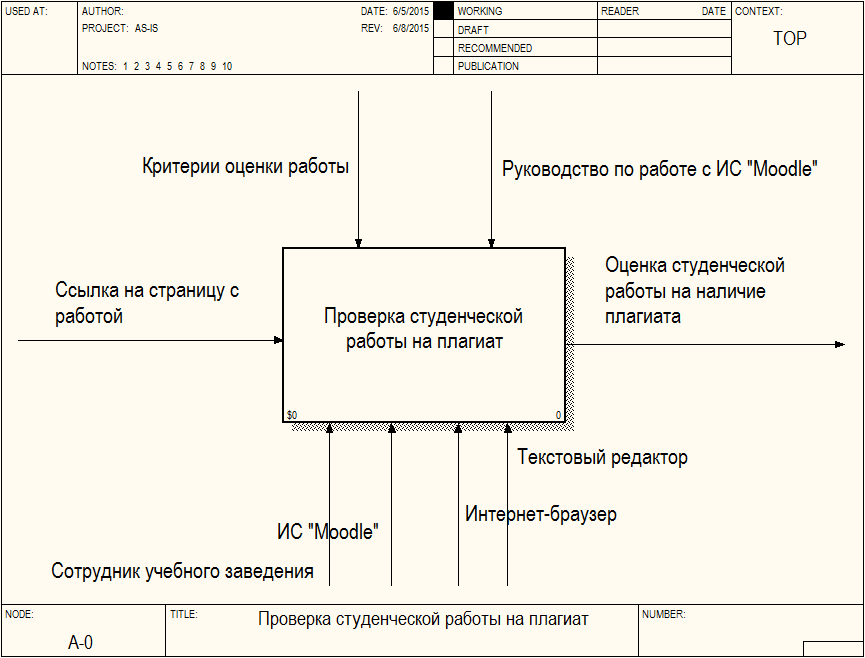
\includegraphics[width=\linewidth]{as_is_context.png}
				  \caption{Контекстная модель процесса до автоматизации}\label{img:as_is_context}
				\endminipage\hfill
				\minipage{0.49\textwidth}
				  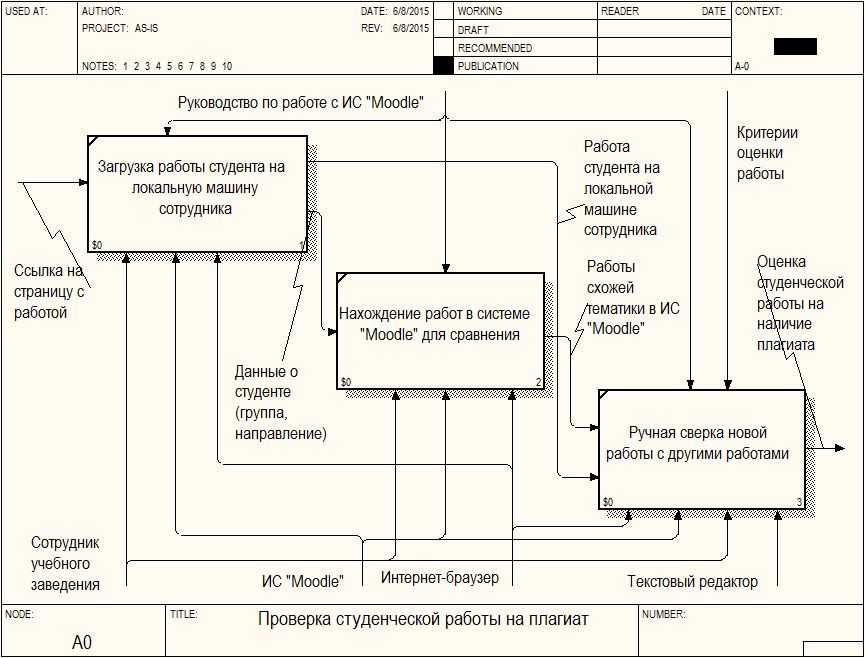
\includegraphics[width=\linewidth]{as_is_decomposition.png}
				  \caption{Декомпозиция контекстной модели}\label{img:as_is_decomposition}
				\endminipage\hfill				
			\end{figure}

			Наиболее трудозатратной операцией в процессе проверки на плагиат для сотрудника является ручная проверка работы на наличие заимствований. В качестве базы для сравнения используются работы всех студентов схожей тематики.			

			На вход в процесс поступает ссылка на документ в системе дистанцтионного обучения, который требуется проверить. Результатом выполнения процесса является оценка работы, исходя из результатов проверки.

		\subsubsection{Модель бизнес-процессов обработки информации («TO--BE»)}

			После анализ функциональной модели «AS--IS» была спроектирована модель «TO--BE», на которой отображается новая модель процесса проверки на плагиат, в которой сотруднику необходимо только принять решение на основе полученных результатов от ИС (степень совпадения и наиболее похожая работа), или запустить проверку, если она ещё не осуществлялась.

			На рисунках \ref{img:to_be_context} и \ref{img:to_be_decomposition} представлены контекстная диаграмма процесса после автоматизации и декомпозиция контекстной диаграммы 1-ого уровня соответственно.
			
			\begin{figure}[h]
				\minipage{0.49\textwidth}
				  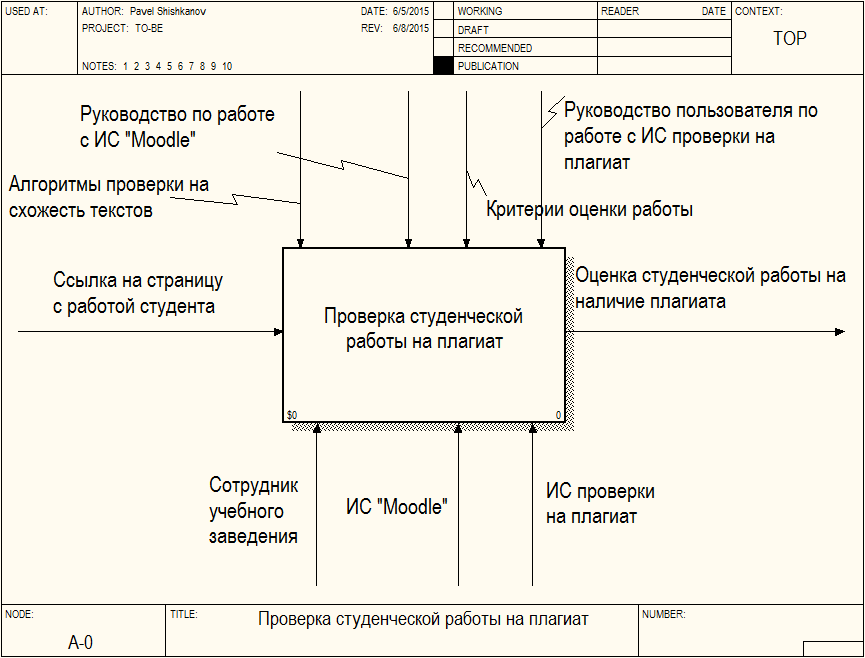
\includegraphics[width=\linewidth]{to_be_context.png}
				  \caption{Контекстная модель процесса после автоматизации}\label{img:to_be_context}
				\endminipage\hfill
				\minipage{0.49\textwidth}
				  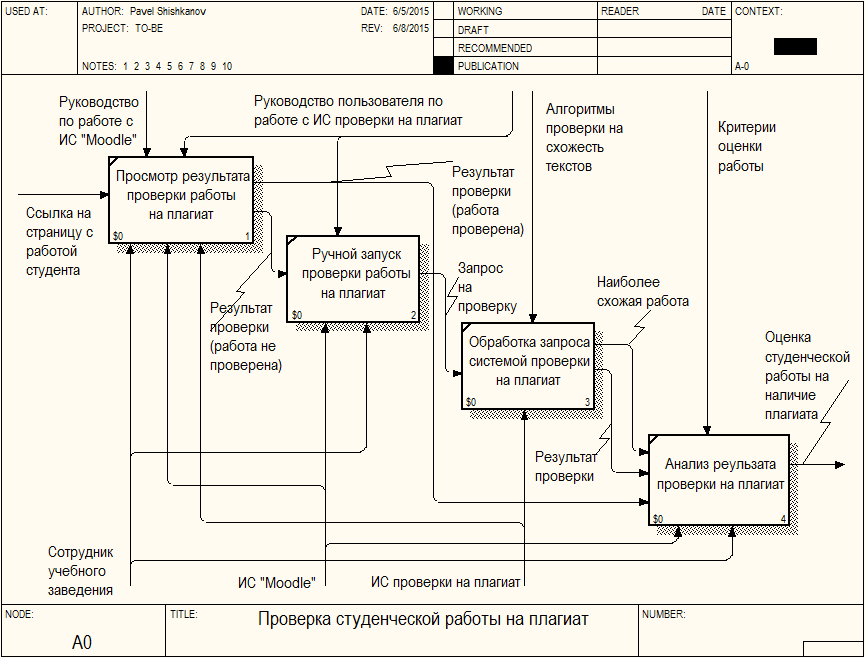
\includegraphics[width=\linewidth]{to_be_decomposition.png}
				  \caption{Декомпозиция контекстной модели}\label{img:to_be_decomposition}
				\endminipage\hfill				
			\end{figure}

	\section{Проектирование ИС}

	При проектировании новой ИС в перую очередь было уделено внимание тому, что разрабатываемая система может использоваться не только в связке с платформой дистанционного обучения, но и как самостоятельная ИС. По этому реализуемая система включает в себя две части: независимая ИС для проверки на плагиат и надстройка в виде плагина для платформы дистанционного обучения.

	Кодовое название ИС: <<Шерлок>>.

	Работа с ИС <<Шерлок>> предпологает два варианта: синхронный и асинхронный. В первом варианте при запросе на проверку клиент будет ожидать результата проверки всё время обработки запроса, а во втором варианте клиенту после первого запроса вернётся ункальный идетификатор проверяемой работы, по которому он в дальшейшем сможет получить результат проверки. В случае, если при проверке работы сотрудником учебного заведения работа ещё не прошла проверку на плагиат, то сотрудник может вручную запустить процесс проверки работы. 

	Интеграция платформы дистанционного обучения Moodle с ИС <<Шерлок>> происходит с помощью плагина, основная задача которого - это регулярная проверка наличия новых работ в системе <<Moodle>> и отправка таких работ на проверку в ИС <<Шерлок>>, а так же отображение результата проверки.

	\subsection{Cистема управления базами данных}

		В качестве СУБД в проекте была выбрана документо-ориентированая база <<MongoDB>> по следующим причинам:
		\begin{itemize}
			\item гибкая модель данных, отличная от той, что предлагают реляционные БД. В ИС <<Шерлок>> модель данных представляет из себя очень ограниченный набор типов объектов и их взаимоотношений между собой, и по этой причне нет необходимости в реляционной алгебре, которая является основой работы традиционных СУБД;
			\item простая установка и настройка. Даже когда появиится потребность в распределённой БД, добавление новых узлов не потребует много усилий;
			\item тестная интеграция с уже существующими технологиями.
		\end{itemize}

	\subsection{Технологии, используемые для реализации ИС}

		В связи с разделением проекта на две части, ИС <<Шерлок>> (``backend'') и плагин для платформы дистанционного обучения (``frontend''), в проекте представлено два технологических стека.

		\subsubsection{ИС <<Шерлок>>}

			В качестве программной платформы для реализации ИС <<Шерлок>> была выбрана платформа ``Java'' по следующим причинам:
			\begin{itemize}
				\item платформа ``Java'' является платформонезависимой, то есть система, написаная на этой платформе может запускаться на огромном числе различных ОС без каких-либо изменений в исходных кодах системы;
				\item за долгое время развития этой платформы было создано огромное число различных готовых инструментов для решения самых различных задач.
			\end{itemize}

			Основной паттерн взаимодействия с ИС - это принятие запроса, его обработка и отправка ответа. Предпологается, что взаимодействие с ИС может происходить из разных сторонних систем, которые могут быть реализованы на совершенно различных технологических стеках. В связи с этим, протокол взаимодействия должет быть таким, который доступен в как можно большем числе технологий. В качестве такого метода взаимодействия был выбран принцип взаимодействия REST на основе протокола HTTP, так как протокол HTTP имеет широкое распространение в Интернете и для работы с ним уже существует большое число готовых решений.

			Для разработки ИС на платформе ``Java'' существует ряд фреймворков, в которых уже реализована часть типовых задач, с которыми чаще всего сталкиваются разработчики. В качестве таких задач могут выступать работа с различными сетевыми протоколами, управление безопастностью приложения, валидация данных, работа с хранилищами данных, поддержка механизма внедрения зависимостей и другие задачи. В данном проекте в качестве такого фреймворка был выбран Spring Framework по ряду причин:
			\begin{itemize}
				\item активная разработка и поддержка этого фреймворка даёт возможность легко использовать многие современные технологии, используемые при разработке ПО;
				\item за долгую историю развития (более 10 лет) вокруг этого фреймворка сформировалось большое сообщество разработчиков и было написано большое число литературы;
				\item данный фреймворк построен по принципу модульности, что позволяет использовать только те части, которые действительно требуются в проекте.
			\end{itemize}

		\subsubsection{Плагин для платформы дистанционного обучения}

			Расширение функционала для ИС <<Moodle>> осуществляется с помощью плагинов, которые описываются на языке программиирования PHP \cite{Moore2010}. 

	\subsection{Сравнение аналогов}

		На данный момент для решения вопроса автоматизации проверки работ на плагиат уже существует ряд систем, наиболее распространённые из которых описываются ниже (JPlag, MOSS).

		JPlag - это система, которая позволяет определять схожесть исходных кодов, написанных на языках Java, C, C++, C\# и Scheme. Так же имеется возможность проверки обычных текстовых документов. Данный сервис доступен как веб-сервис. В качестве алгоритма сравнения работ JPlag использует алгоритм <<greedy string tiling>> \cite{Wise1993}. При использовании этого алгоритма его сложность в худшем случае - $O(n^3)$, а в лучшем - $O(n^2)$ \cite{Prechelt2002}.  Для повышения эффективности работы алгоритма проверки применяется алгоритм Рабина — Карпа \cite{Burrows2007} \cite{Karp1987}, с которым сложность становится почти линейной - $O(n^{1,12})$. Результат сравнения представляется в виде HTML-страницы, на которой отображаются заимствованные части проверяемой работы.

		MOSS (Measure Of Software Similarity) - система проверки на плагиат, доступная как веб-сервис. Имеется возможность проверки работ на таких языках программирования, как Java, C, C++, Scheme. В качестве методов для сверки работ используются <<fingerprinting technique>> и алгоритм <<Winnowing>> \cite{Winnowing2003}.		

		В ходе анализа уже существующих решений был определён ряд требований, которыми в совокупности не обладает ни одна из рассмотренных систем:
		\begin{itemize}
			\item независимость от третьих лиц и возможность установки системы в рамках университета, для полного контроля над нею;
			\item возможность проверки различных типов текстовых документов;
			\item расширяемость функционала - возможность определения алгоритмов, которые используются для проверки и добавление новых типов проверяемых работ (разные языки программирования);
			\item простота использования для конечного пользователя - сотрудника учебного заведения.
		\end{itemize}

	\subsection{Визуальное проектирование ИС}

		Для лучшего понимания тех или иных аспектов в работе и структуре ИС был разработан ряд диаграмм с использованием нотации UML \cite{Fowler2003}.

		\subsubsection{Диаграмма прецедентов}

			Для определения круга задач, решаемых с помощью разрабатываемой системой с точки зрения пользователя, была разработана диаграмма прецедентов (рис. \ref{img:use_case_diagram}), на которой отображены основные пользователи, взаимодействующие с системой, а также возможности, доступные для них.
			\newline
			\newline
			\begin{figure}[h]
				\center{\frame{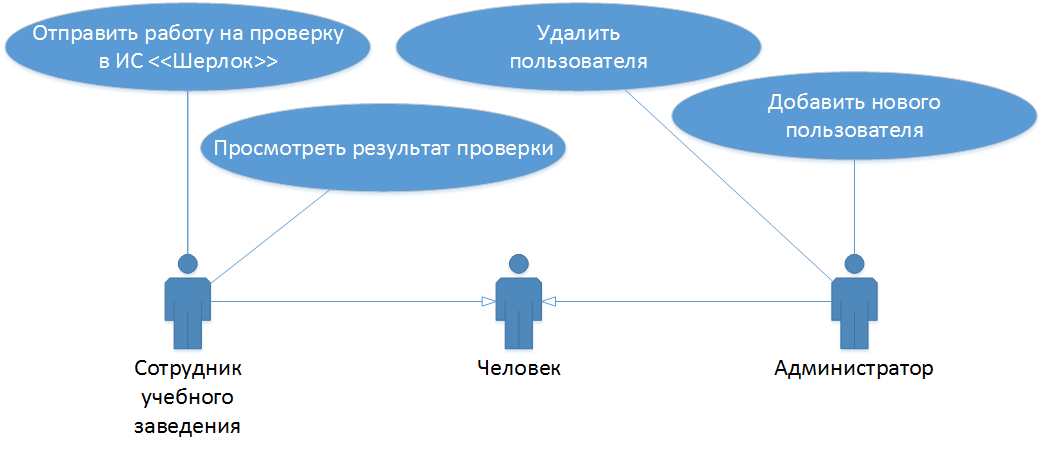
\includegraphics[width=0.8\linewidth]{use_case_diagram.png}}}
				\caption{Диаграмма прецедентов}
				\label{img:use_case_diagram}
			\end{figure}
			
			Описание прецедентов:
			\begin{itemize}
				\item ``Отправить работу на проверку в ИС <<Шерлок>>'' \\
				Предусловие: нахождение на странице проверяемой работы. \\
				Действующее лицо: сотрудник учебного заведения. \\
				Основной поток: отправка работы на проверку на плагиат. \\
				Альтернативный поток: в ходе проверки возникла ошибка. Необходима ручная проверка. \\
				Описание: сотрудник отправляет работу на проверку в ИС <<Шерлок>> на выявление факта плагиата. \\
				Постусловие: работа отправлена на проверку. \\

				\item ``Просмотереть результаты проверки'' \\
				Предусловие: нахождение на странице работы, для которой был получен результат проверки. \\
				Действующее лицо: сотрудник учебного заведения. \\
				Основной поток: просмотр результата проверки. \\
				Альтернативный поток: результат проверки не представлен. Необходима ручная проверка. \\
				Описание: сотрудник просматривает результаты проверки работы на плагиат, для которой он отправлял запрос. \\
				Постусловие: сотрудник просмоетрел результат. \\

				\item ``Добавить нового пользователя'' \\				
				Действующее лицо: администратор. \\
				Основной поток: добавление новго пользователя в ИС <<Шерлок>>. \\
				Альтернативный поток: новый пользователь не добавлен. Попробывать ещё раз с новыми данными о пользователе. \\
				Описание: администратор добавляет нового пользователя в ИС <<Шерлок>>, что бы тот смог отправлять работы на проверку и просматривать результаты проверки. \\
				Постусловие: в ИС <<Шерлок>> добавлен новый пользователь. \\

				\item ``Удалить пользователя'' \\				
				Действующее лицо: администратор. \\
				Основной поток: удаление пользователя из ИС <<Шерлок>>. \\
				Альтернативный поток: удаление не выполнено. Попробывать ещё раз с новыми данными о пользователе. \\
				Описание: администратор пользователя из ИС <<Шерлок>>. \\
				Постусловие: пользователь удалён из ИС <<Шерлок>>.
			\end{itemize}

		\subsubsection{Диаграмма классов}

			Для описания модели объектов и их взаимодействия между собой была составлена диаграмма классов (рис. \ref{img:class_diagram}).
			\newline
			\begin{figure}[h]
				\center{\frame{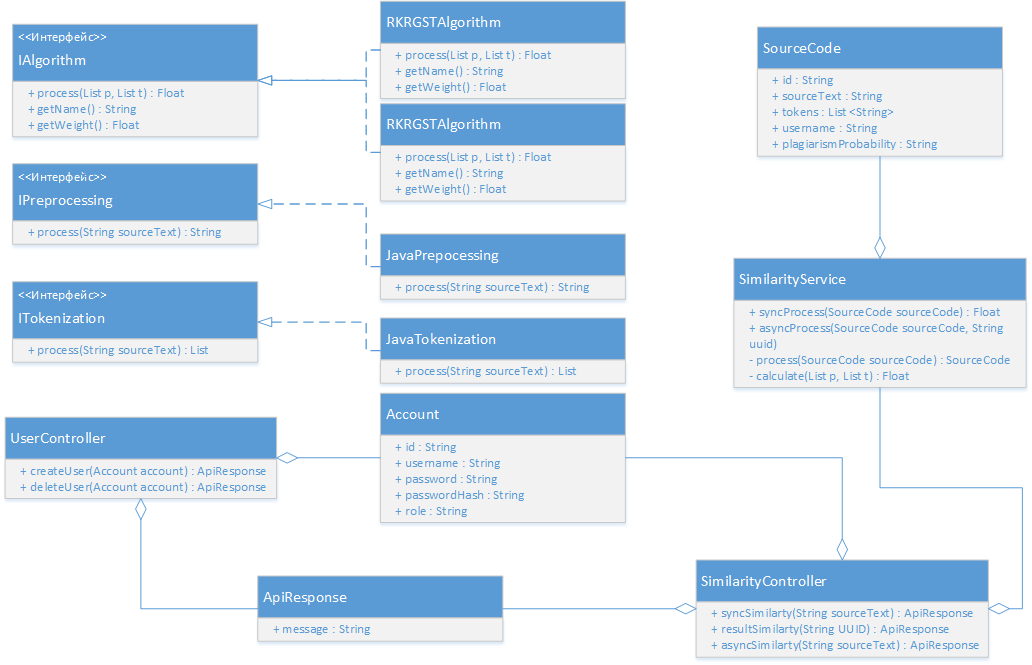
\includegraphics[width=0.9\linewidth]{class_diagram.png}}}
				\caption{Диаграмма классов}
				\label{img:class_diagram}
			\end{figure}

		\newpage
		\subsubsection{Диаграмма последовательности}

			На рис. \ref{img:sequence_diagram} представлена диаграмма последовательности, которая описывает наиболее частый сценарий использования ИС - обработка синхронного запроса на проверку работы.	
			\newline
			\begin{figure}[h]
				\center{\frame{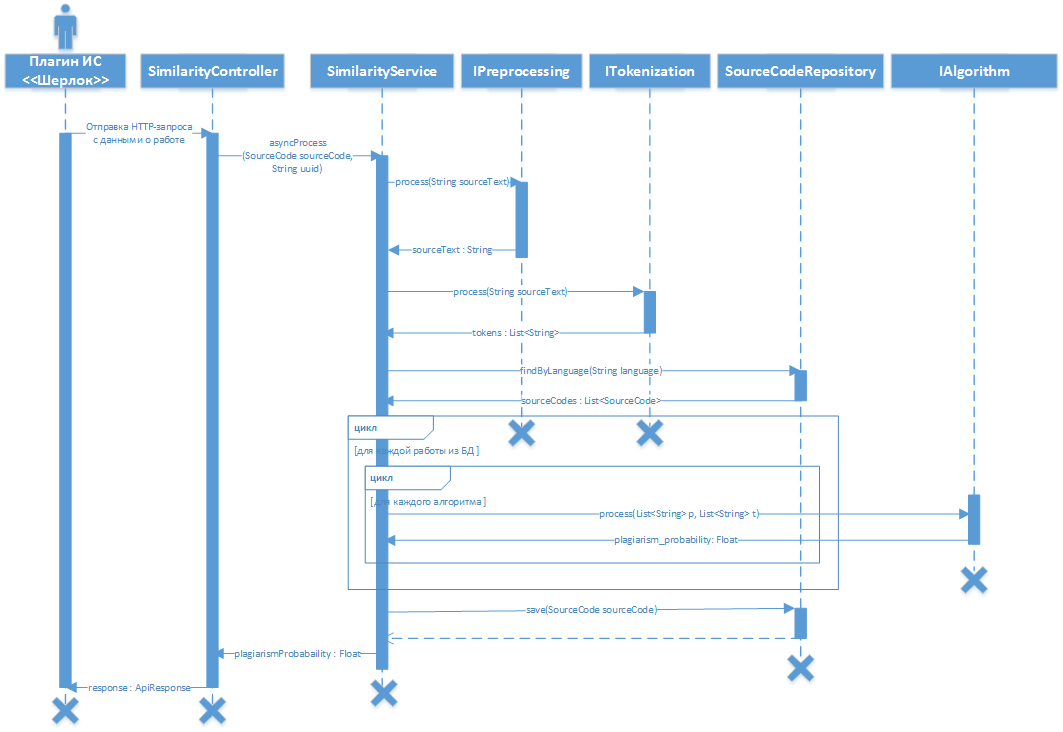
\includegraphics[width=0.95\linewidth]{sequence_diagram.png}}}
				\caption{Диаграмма последовательности}
				\label{img:sequence_diagram}
			\end{figure}

		\newpage
		\subsubsection{Диаграмма развёртывания}

			На рис. \ref{img:deployment_diagram} представлена диаграмма развёртывания, на которой отображено взаимодействие между разными компонентами ИС.
			\newline
			\begin{figure}[h]
				\center{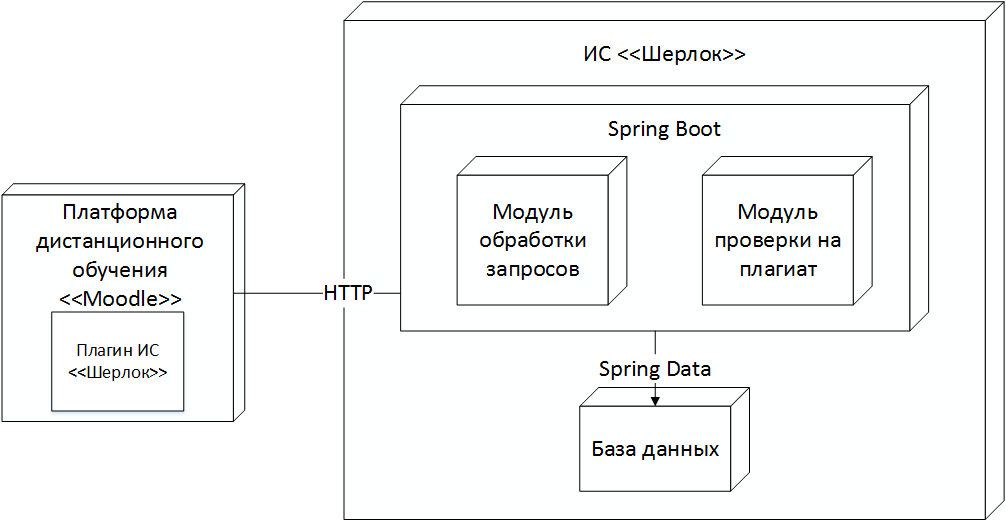
\includegraphics[width=0.95\linewidth]{deployment_diagram.png}}
				\caption{Диаграмма последовательности}
				\label{img:deployment_diagram}
			\end{figure}
	\section{Реализация прототипа ИС}
	
	\subsection{Cостав и структура команды разработки}

		Для разработки ИС была укомплектована команда, состоящя из следующих участиков:
		\begin{itemize}			
			\item прикладной математик;
			\item проектировщик;
			\item разработчик (backend);
			\item разработчик (fronend);
			\item тестировщик.
		\end{itemize}

		Задача прикладного математикак - реализация необходимых алгоритмов для выявления совпадений в документах.

		Задача проектировщика - разработать архитектуру будущей ИС и выбор технологий для реализации ИС.

		Задача разработчика (backend) - реализация ИС с учётом выбранной архитектуры и технологий, а так же с использованием наработок математика.

		Задача разработчика (fronend) - реализация плагина для ИС <<Moodle>>, который предоставляет интерфейс для работы с ИС <<Шерлок>>.

		Задача тестировщика - проверка корректности работы ИС и проверка на соответствие с требованиями.

	\subsection{Выбор и описание средств владения кода}

		В качестве системы управления версиями исходного кода был выбран Git - эта система получшила широкое распространение и интеграцию в сторонние продукты, содержит необходимый функционал, а так же бесплатна. 

	\subsection{Алгоритмы, использумые в разработке ИС.}

		Для выявления схожести между документами применяется несколько алгоритмов, но не один из них не является лучшим для проверки разных типов работ. В текущей версии ИС <<Шерлок>> используются только один алгоритм: RKR-GST (Running-Karp-Rabin Greedy-String-Tiling) \cite{Wise1993}. В дальнейшем будет добавлен алгоритм Winnowing \cite{Winnowing2003}:

		\subsubsection{Описание алгоритма RKR-GST}

			Данный алгоритм состоит из двух этапов. На первом этапе происходит поиск наиболее длинной последовательности в обеих документах. Для поиска совпадений используется алгоритм Рабина — Карпа \cite{Karp1987} и длина совпадения должна быть больше минимального значения, заданного изначально. На втором этапе совпадения помечаются, что бы в дальнейшем уже найденные совпадения не использовались на первом этапе при последующих итерациях. После того, как все совпадения будут помечены, первый этап алгоритма начинается снова. Алгоритм завершается в том случае, когда длина найденного совпадения меньше минимального значения, заданного изначально. В приложении Б представлен псевдокод данного алгоритма.

	\newpage
	\subsection{Этапы обработки запроса}

		Процесс обработки запроса на проверку на плагиат состоит из нескольких этапов:
		\begin{itemize}			
			\item препроцессинг;
			\item токенизация;
			\item вычисление схожести;
			\item вычисление итогового результата.
		\end{itemize}

		Качество реализации этапов препроцессинга и токенизации играет большое влияние на итоговый результат проверки на схожесть работ \cite{Kleiman2009}. 

		\subsubsection{Препроцессинг}

			На данном этапе происходит ``очистка'' проверяемой работы от таких изменений, как удаление комментариев, разделение или слияние блоков определения переменных, изменения порядка определения переменных, добавление лишних операторов. Такие изменения вносятся в исходную работу студентом с целью снижения вероятности обнаружения плагиата в работе.

		\subsubsection{Токенизация}

			На данном этапе происходит преобразование проверяемой работы в набор токенов. Например, все значения и переменные заменяются на токены <IDENT> и <VALUE> соответственно. Данный процесс позволяет преобразовать работу в такой формат, с котором наиболее эффективно работают алгоритмы сравнения. В данной работе для токенизации используется библиотека ANTLR \cite{Parr2013}.

		\subsubsection{Вычисление схожести}

			На данном этапе происходит сравнение работы из запроса с работами, которые хранятся в БД. Для сравнения отбираются не все работы, а только те, которые имеют схожую тематику с проверяемой работой. При сравнении вычисляется значение схожести с использованием каждого алгоритма по отдельности.

			Для алгоритма RKR-GST значение схожести между работами определяется по формуле \ref{eq:sim}.
			\begin{equation}\label{eq:sim}
				sim(a,b) = \frac{ 2 * coverage }{ length(a) + length(b) },
			\end{equation}
			\begin{ESKDexplanation}
				\item[где ] $length(a)$ --- число токенов в работе $a$;
				\item$length(b)$ --- число токенов в работе $b$;
				\item$coverage$ --- число совпадений в работах.		
			\end{ESKDexplanation}

		\subsubsection{Вычисление итогового результата}		

			Итоговый результат проверки опрелеяется по формуле \ref{eq:result_sim}.

			\begin{equation}\label{eq:result_sim}
				sim(a,b) = \sum_{i=1}^{n} \frac{ w_i * sim_i(a,b) }{ w },				 
			\end{equation}
			\begin{ESKDexplanation}
				\item[где ] $sim_i$ --- рассчитанное значение схожести между работами для алгоритма i;
				\item$w_i$ --- вес алгоритма;
				\item$w$ --- общий вес всех алгоритмов;
				\item$n$ --- число используемых алгоритмов при проверке.		
			\end{ESKDexplanation}



	\section{Имитационное моделирование}

	В начале эксплуатации ИС <<Шерлок>> в реальных условиях обработка запросов может происходить за допустимое время, но с ростом базы знаний ИС (при каждом запросе после обработки происходит сохранение проверенной работы в БД) и числа пользователей (потонциальный функционал ИС не ограничен проверкой исходных кодов программ, и может использоваться для проверок любых типов работ, что влечёт за собой расширение круга пользователе ИС) время обработки будет увеличиваться, что может отрицательно сказаться на работе тех систем, которые взаимодействуют с ИС <<Шерлок>>.

	Для определения времени обработки работы при заданном числе запросов за единицу времени была разработана иммитационная модель в среде AnyLogic. Графическое изображение этой модели представленно на рис. \ref{img:simulation_model}.

	\begin{figure}[h]
		\center{\frame{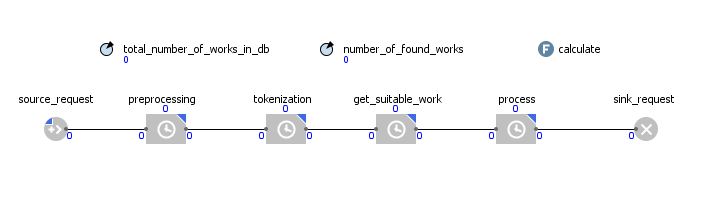
\includegraphics[width=0.8\linewidth]{simulation_model.png}}}1
		\caption{Имитационная модель обработки запроса}
		\label{img:simulation_model}
	\end{figure}

	Весь цикл обработки запроса состоит из нескольких операций, которые занимают разное количество времени:
	\begin{itemize}
		\item preprocessing - этап, на котором происходит ``очистка'' работы студента от той информации, которая ухудшает качество проверки;
		\item tokenization - этап, на котором происходит разбор исходной работы на токены, на основе которых происходит дальнейшее сравнение работ; время операции зависит от типа работы, так как обработка работ на разных языках программирования имеет различную сложность;
		\item get-suitable-work - этап, на котором происходит выборка работ из БД схожей тематики с работой, присланной на проверку;
		\item process - этап, на котором происходит сравнение найденых работ из БД с проверяемой работой; время операции зависит от числа работ, найденых для сравнения и от сложности алгоритмов, используемых при проверке.
	\end{itemize}

	В переменнах total-number-of-works-in-db и number-of-found-works хранится общее число работ в БД и число работ, найденных для сравнения с проверяемой работой соответственно.

	Время сравнения работ выисляется с помощью функции calculate. В теле этой функции считается время, затраченное на поочерёдное сравнение работ с помощью каждого алгоритма, который реализован в системе.

	Для определения конкретных значений времени обработки для каждого из этапов было произведено тестирование прототипа ИС, в результате чего были получены следующие значения:
	\begin{itemize}
		\item preprocessing - случайное значение в пределах от 10 до 20 мс;
		\item tokenization - размер проверяемой работы в байтах умноженное на случайное значение в пределах от 0,1 до 0,2 мс;
		\item get-suitable-work - общее число работ в БД умноженное на 0.0000313 мс (такое среднее время было полученно для чтения одной записи);
		\item process - сумма времени сравнения каждой найденой записи с проверяемой работой по каждому из алгоритмов.
	\end{itemize}

	После проведения тестов на разработанной модели можно определить, какой из этапов обработки является узким местом в системе. В зависимости от типа найденой проблемы можно предложить ряд мер, направленных на её устранение:
	\begin{itemize}
		\item программная реализация паралеллизма обработки запросов;
		\item уменьшение сложности применяемых алгоритмов путём применения различных эвристик;
		\item улучшение алгоритма выборки подходящих работ для сравнения.		
	\end{itemize}


	\section{Информационный менеджмент}

	\subsection{Ресурсная матрица проекта}

	Целью создания данной ИС служит автоматизация процесса проверки работ на плагиат. Оценку эффективности внедрения ИС можно проводить по нескольким показателям, в том числе и по сокращению временных затрат. Для этого необходимо построить ресурсные матрицы для процесса до и после автоматизации, и на их основе рассчитать эффективность от внедрения.

		\subsubsection{Ресурсная матрица процесса до автоматизации}	

			Процесс проверки работы на плагиат до автоматизации состоял из следующих операций:
			\begin{itemize}
				\item загрузка работы студента на локальную машину сотрудника;
				\item нахождение работ в системе <<Moodle>> для сравнения;
				\item ручная сверка новой работы с другими работами.
			\end{itemize}

			В таблице \ref{tab:resources_before} представлены ресурсы, которые используются в процессе до автоматизации.

			\begin{table}[h]
				\centering
				\caption{Ресурсная матрица процесса до автоматизации}
				\label{tab:resources_before}				
				\begin{tabular}{|l|l|l|}
				\hline
					\multicolumn{1}{|c|}{$Р_{Сотр}$} 				&
					\multicolumn{1}{ c|}{$Р_{\text{Сотр-Moodle}}$} 	&
					\multicolumn{1}{ c|}{$Р_{\text{Сотр-Local}}$} 	\\ \hline
					\multicolumn{1}{|c|}{$Р_{\text{Сотр-Moodle}}$} 	&
					\multicolumn{1}{ c|}{$Р_{\text{Moodle}}$} 		&
					\multicolumn{1}{ c|}{$-$} 						\\ \hline
					\multicolumn{1}{|c|}{$Р_{\text{Сотр-Local}}$} 	&
					\multicolumn{1}{ c|}{$-$} 						&
					\multicolumn{1}{ c|}{$Р_{\text{Local}}$}			\\ \hline                           
				\end{tabular}
			\end{table}			

			\newpage
			В таблице \ref{tab:resources_ref_before} приведено описание ресурсов из таблицы \ref{tab:resources_before}.

			\begin{table}[h]
				\small
				\centering
				\caption{Компоненты ресурсной матрицы до автоматизации}
				\label{tab:resources_ref_before}				
				\begin{tabular}{|l|l|}				
				\hline
					\multicolumn{1}{|c|}{Ресурс} 										&
					\multicolumn{1}{ c|}{Описание} 										\\ \hline
					$Р_{\text{Сотр}}$													&
					Сотрудник учебного заведения (25\,000 руб./мес. или 142 руб./час) 	\\ \hline
					$Р_{\text{Moodle}}$													&
					Рабочая станция с установленной ИС <<Moodle>> (30\,000 руб.) 		\\ \hline
					$Р_{\text{Local}}$													&
					Рабочая станция сотрудника (25\,000 руб.)							\\ \hline
					$Р_{\text{Сотр-Moodle}}$											&
					Взаимодействие сотрудника с ИС <<Moodle>> (180 мин./день)			\\ \hline
					$Р_{\text{Сотр-Local}}$												&
					Рабочий процесс сотрудника на локальном ПК (30 мин./день)			\\ \hline
				\end{tabular}
			\end{table}			

			В качестве значений для ресурсов $Р_{\text{Moodle}}$ и $Р_{\text{Local}}$ рассчитывается амортизация этого оборудования за месяц - 500 руб. и 415 руб. соответственно.

			Значение для ресурса $Р_{\text{Сотр-Moodle}}$ рассчитывается как 180 * 3 * 4 = 21 час/мес., так как в среднем сотрудник проверяет работы 3-х групп за неделю. Соответственно, значение для $Р_{\text{Сотр-Local}}$ определяется как 30 * 3 * 4 = 6 часов/мес.			

			\begin{table}[h]
				\centering
				\caption{Временная ресурсная матрица до автоматизации}
				\label{tab:time_resources_before}				
				\begin{tabular}{|l|l|l|}
				\hline
					\multicolumn{1}{|c|}{25\,000} 	&
					\multicolumn{1}{ c|}{2\,982 } 	&
					\multicolumn{1}{ c|}{852} 		\\ \hline
					\multicolumn{1}{|c|}{2\,982} 	&
					\multicolumn{1}{ c|}{500} 		&
					\multicolumn{1}{ c|}{0} 			\\ \hline
					\multicolumn{1}{|c|}{852} 		&
					\multicolumn{1}{ c|}{0} 			&
					\multicolumn{1}{ c|}{415}		\\ \hline                           
				\end{tabular}
			\end{table}	

			\begin{table}[h]
				\centering
				\caption{Нормированная временная ресурсная матрица до автоматизации}
				\label{tab:normalization_time_resources_before}				
				\begin{tabular}{|l|l|l|}
				\hline
					\multicolumn{1}{|c|}{1,000} 	&
					\multicolumn{1}{ c|}{0,119} 		&
					\multicolumn{1}{ c|}{0,034} 		\\ \hline
					\multicolumn{1}{|c|}{0,119} 	&
					\multicolumn{1}{ c|}{0,020} 		&
					\multicolumn{1}{ c|}{0,000} 		\\ \hline
					\multicolumn{1}{|c|}{0,034} 	&
					\multicolumn{1}{ c|}{0,000} 		&
					\multicolumn{1}{ c|}{0,016}		\\ \hline                           
				\end{tabular}
			\end{table}								

			В таблице \ref{tab:time_resources_before} представлены сводные значения по ресурсам, а в таблице \ref{tab:normalization_time_resources_before}  приведены значения после нормировкии относительно ресурса $Р_{\text{Сотр}}$.

			\newpage
			В таблице \ref{tab:resource_costs_before} приведены коэффициенты использования каждого ресурса по операциям.

			\begin{table}[h]
				\small
				\centering
				\caption{Затраты ресурсов на выполнение операций до автоматизации}
				\label{tab:resource_costs_before}				
				\begin{tabular}{|l|l|l|l|}				
				\hline
					\multicolumn{1}{|c|}{Ресурсы} 										&
					\multicolumn{1}{ c|}{Операция 1} 									&
					\multicolumn{1}{ c|}{Операция 2} 									&
					\multicolumn{1}{ c|}{Операция 3} 									\\ \hline
					$Р_{\text{Сотр}}$													&
					\multicolumn{1}{ c|}{0,05}											&
					\multicolumn{1}{ c|}{0,10}																&
					\multicolumn{1}{ c|}{0,85}																\\ \hline
					$Р_{\text{Moodle}}$													&
					\multicolumn{1}{ c|}{0,10}																&
					\multicolumn{1}{ c|}{0,50}															&
					\multicolumn{1}{ c|}{0,40}																\\ \hline
					$Р_{\text{Local}}$													&
					\multicolumn{1}{ c|}{0,20}															&
					\multicolumn{1}{ c|}{0,00}																&
					\multicolumn{1}{ c|}{0,80}																\\ \hline
					$Р_{\text{Сотр-Moodle}}$											&
					\multicolumn{1}{ c|}{0,10}																&
					\multicolumn{1}{ c|}{0,80}																&
					\multicolumn{1}{ c|}{0,10}																\\ \hline
					$Р_{\text{Сотр-Local}}$												&
					\multicolumn{1}{ c|}{0,20}																&
					\multicolumn{1}{ c|}{0,00}																&
					\multicolumn{1}{ c|}{0,80}																\\ \hline
				\end{tabular}
			\end{table}

			Для оценки качества работы ИС и объема выполненных ею работ необходимо определить некоторые количественные меры, что позволит корректно вычислять соответствующие функционалы, например взвешенную сумму $Ф_к$ затраченных на выполнение k-ого технологического процесса ресурсов вида \ref{eq:functional_before}:
			\begin{equation}\label{eq:functional_before}
				Ф_к = (\sum_{r=1}^{m_k} f_r Р_r)_к,				
			\end{equation}
			\begin{ESKDexplanation}
				\item[где ] $r$ 		--- индекс суммирования затрат составляющих ресурсов по k-ому технологическому маршруту;
				\item $m_k$ --- число операций k-ого технологического процесса;
				\item $f_r$ --- весовой коэффициент r-ого компонента ресурса.
			\end{ESKDexplanation}

			Расчет эффективности для описанного процесса:

			$Ф_1 = 0,05 * 1,000 + 0,10 * 0,020 + 0,20 * 0,016 + 0,10 * 0,119 + 0,20 * 0,034 = 0,074;$

			$Ф_2 = 0,10 * 1,000 + 0,50 * 0,020 + 0,80 * 0,119 = 0,205;$

			$Ф_3 = 0,85 * 1,000 + 0,40 * 0,020 + 0,80 * 0,016 + 0,10 * 0,119 + 0,80 * 0,034 = 0,910;$

			$Ф = 1,189.$

		\subsubsection{Ресурсная матрица процесса после автоматизации}	

			Процесс проверки работы на плагиат после автоматизации состоит из следующих операций:
			\begin{itemize}
				\item обработка запроса системой проверки на плагиат;
				\item просмотр результата проверки работ на плагиат;				
				\item анализ результата проверки.
			\end{itemize}

			В таблице \ref{tab:resources_after} представлены ресурсы, которые используются в процессе после автоматизации.

			\begin{table}[h]
				\centering
				\caption{Ресурсная матрица процесса после автоматизации}
				\label{tab:resources_after}				
				\begin{tabular}{|l|l|l|}
				\hline
					\multicolumn{1}{|c|}{$Р_{Сотр}$} 				&
					\multicolumn{1}{ c|}{$Р_{\text{Сотр-Moodle}}$} 	&
					\multicolumn{1}{ c|}{$-$} 	\\ \hline
					\multicolumn{1}{|c|}{$Р_{\text{Сотр-Moodle}}$} 	&
					\multicolumn{1}{ c|}{$Р_{\text{Moodle}}$} 		&
					\multicolumn{1}{ c|}{$-$} 						\\ \hline
					\multicolumn{1}{|c|}{$-$} 	&
					\multicolumn{1}{ c|}{$-$} 						&
					\multicolumn{1}{ c|}{$Р_{\text{Шерлок}}$}			\\ \hline                           
				\end{tabular}
			\end{table}					
			
			В таблице \ref{tab:resources_ref_after} приведено описание ресурсов из матрицы.

			\begin{table}[h]
				\small
				\centering
				\caption{Компоненты ресурсной матрицы после автоматизации}
				\label{tab:resources_ref_after}				
				\begin{tabular}{|l|l|}				
				\hline
					\multicolumn{1}{|c|}{Ресурс} 										&
					\multicolumn{1}{ c|}{Описание} 										\\ \hline
					$Р_{\text{Сотр}}$													&
					Сотрудник учебного заведения (25\,000 руб./мес. или 142 руб./час) 	\\ \hline
					$Р_{\text{Moodle}}$													&
					Рабочая станция с установленной ИС <<Moodle>> (30\,000 руб.) 		\\ \hline
					$Р_{\text{Шерлок}}$													&
					Рабочая станция с ИС <<Шерлок>> (25\,000,00 руб.)					\\ \hline
					$Р_{\text{Сотр-Moodle}}$											&
					Взаимодействие сотрудника с ИС <<Moodle>> (10 мин./день)			\\ \hline
				\end{tabular}
			\end{table}		

			В качестве значений для ресурсов $Р_{\text{Moodle}}$ и $Р_{\text{Шерлок}}$ рассчитывается амортизация этого оборудования за месяц - 500,00 руб. и 415,00 руб. соответственно.

			Значение для ресурса $Р_{\text{Сотр-Moodle}}$ рассчитывается как 20 * 3 * 4 = 2 часа/мес., так как в среднем сотрудник проверяет работы 3-х групп за неделю.

			\newpage
			В таблице \ref{tab:time_resources_after} представленны сводные значения по ресурсам, а в таблице \ref{tab:normalization_time_resources_after}  приведены значения после нормировкии относительно ресурса $Р_{\text{Сотр}}$.

			\begin{table}[h]
				\centering
				\caption{Временная ресурсная матрица после автоматизации}
				\label{tab:time_resources_after}				
				\begin{tabular}{|l|l|l|}
				\hline
					\multicolumn{1}{|c|}{25\,000} 	&
					\multicolumn{1}{ c|}{284 } 	&
					\multicolumn{1}{ c|}{0} 		\\ \hline
					\multicolumn{1}{|c|}{284} 	&
					\multicolumn{1}{ c|}{500} 		&
					\multicolumn{1}{ c|}{0} 			\\ \hline
					\multicolumn{1}{|c|}{0} 		&
					\multicolumn{1}{ c|}{0} 			&
					\multicolumn{1}{ c|}{415}		\\ \hline                           
				\end{tabular}
			\end{table}	

			\begin{table}[h]
				\centering
				\caption{Нормированная временная ресурсная матрица после автоматизации}
				\label{tab:normalization_time_resources_after}				
				\begin{tabular}{|l|l|l|}
				\hline
					\multicolumn{1}{|c|}{1,000} 	&
					\multicolumn{1}{ c|}{0,011} 		&
					\multicolumn{1}{ c|}{0,000} 		\\ \hline
					\multicolumn{1}{|c|}{0,011} 	&
					\multicolumn{1}{ c|}{0,020} 		&
					\multicolumn{1}{ c|}{0,000} 		\\ \hline
					\multicolumn{1}{|c|}{0,000} 	&
					\multicolumn{1}{ c|}{0,000} 		&
					\multicolumn{1}{ c|}{0,016}		\\ \hline                           
				\end{tabular}
			\end{table}				

			В таблице \ref{tab:resource_costs_after} приведены коэффициенты использования каждого ресурса по операциям.

			\begin{table}[h]
				\small
				\centering
				\caption{Затраты ресурсов на выполнение операций после автоматизации}
				\label{tab:resource_costs_after}				
				\begin{tabular}{|l|l|l|l|}				
				\hline
					\multicolumn{1}{|c|}{Ресурсы} 										&
					\multicolumn{1}{ c|}{Операция 1} 									&
					\multicolumn{1}{ c|}{Операция 2} 									&
					\multicolumn{1}{ c|}{Операция 3} 									\\ \hline
					$Р_{\text{Сотр}}$													&
					\multicolumn{1}{ c|}{0,00}																&
					\multicolumn{1}{ c|}{0,30}																&
					\multicolumn{1}{ c|}{0,70}																\\ \hline
					$Р_{\text{Moodle}}$													&
					\multicolumn{1}{ c|}{0,20}																&
					\multicolumn{1}{ c|}{0,70}																&
					\multicolumn{1}{ c|}{0,10}																\\ \hline
					$Р_{\text{Шерлок}}$													&
					\multicolumn{1}{ c|}{1,00}																&
					\multicolumn{1}{ c|}{0,00}																&
					\multicolumn{1}{ c|}{0,00}																\\ \hline
					$Р_{\text{Сотр-Moodle}}$											&
					\multicolumn{1}{ c|}{0,00}																&
					\multicolumn{1}{ c|}{0,80}																&
					\multicolumn{1}{ c|}{0,20}																\\ \hline	
				\end{tabular}
			\end{table}								

			Для оценки качества работы ИС и объема выполненных ею работ необходимо определить некоторые количественные меры, что позволит корректно вычислять соответствующие функционалы, например взвешенную сумму $Ф_к$ затраченных на выполнение k-ого технологического процесса ресурсов вида \ref{eq:functional_after}:
			\begin{equation}\label{eq:functional_after}
				Ф_к = (\sum_{r=1}^{m_k} f_r R_r)_к,				
			\end{equation}
			\begin{ESKDexplanation}
				\item[где ] $r$ --- индекс суммирования затрат составляющих ресурсов по k-ому технологическому маршруту;
				\item $m_k$ --- число операций k-ого технологического процесса;
				\item $f_r$ --- весовой коэффициент r-ого компонента ресурса.
			\end{ESKDexplanation}

			Расчет эффективности для описанного процесса:
			$Ф_1 = 0,20 * 0,020 + 1,00 * 0,16  = 0,158; $

			$Ф_2 = 0,30 * 1,000 + 0,70 * 0,020 + 0,80 * 0,016 = 0,318; $

			$Ф_3 = 0,70 * 1,000 + 0,10 * 0,020 + 0,20 * 0,011 = 0,704; $

			$Ф = 1,180. $			

			Исходя из результатов вычислений, можно сделать вывод о том, что внедрение ИС незначительно повысит эффективность процесса.

	\subsection{Экономическое обоснование проекта}

	Для определения экономического обоснования разработки ИС <<Шерлок>> использовались методы функционально-стоимостного анализа. Объектами исследования при таком подходе являются выполняемые функции, а не итоговый результат процесса.

	В качестве оценки экономического обоснования разработки ИС используется коэффициент экономической эффективности. Для расчёта данного коэффициента необходимо рассчитать следующие параметры:
	\begin{itemize}
		\item стоимость разработки ИС;
		\item стоимость выполнения процесса до автоматизации;
		\item стоимость выполнения процесса после автоматизации.
	\end{itemize}

		\subsubsection{Расчет стоимости разработки ИС}

			Стоимость разработки и внедрения ИС складывается из следующих составляющих: 
			\begin{itemize}
				\item затраты на заработную плату участникам процесса разработки системы;
				\item затраты на расходные материалы; 
				\item расходы на амортизацию оборудования и нематериальных активов.
			\end{itemize}

			\indent Стоимость разработки ИС рассчитывается по следующей формуле:
			\begin{equation}\label{eq:cost_of_development}
				С_{ис} = \text{З} + \text{М} + \text{А},
			\end{equation}
			\begin{ESKDexplanation}
				\item[где ] $\text{С}_{\text{ис}}$ 	--- стоимость ИС, руб.;
				\item $\text{З}$ --- затраты на заработную плату специалистам, задействованным в разработке системы, руб.;
				\item $\text{М}$ 			--- затраты на расходные материалы, необходимые при разработке системы, руб.;
				\item $\text{А}$ 			--- амортизация оборудования и нематериальных активов, используемых в процессе разработки ИС, руб..
			\end{ESKDexplanation}


			\indent Для расчета затрат на выплату заработной платы специалистам состовляется квалификационный план проекта разработки системы (таблица \ref{tab:qualification_plan}):


			\begin{table}[h]
				\small
				\centering
				\caption{Квалификационный план проекта разработки ИС}
				\label{tab:qualification_plan}								
				\begin{tabular}{|l|l|p{7cm}|}				
				\hline
					\multicolumn{1}{|c|}{Наименование специалиста} 							&
					\multicolumn{1}{ c|}{Величина ставки (руб.)} 							&
					\multicolumn{1}{ c|}{Выполняемые функции} 								\\ \hline
					Прикладной математик 													&
					\multicolumn{1}{ c|}{60\,000}																&
					Реализация необходимых математических алгоритмов						\\ \hline
					Проектировщик 															&
					\multicolumn{1}{ c|}{65\,000}																	&
					Определение архитектуры будующей ИС, используемых паттернов и технологий\\ \hline
					Разработчик (``backend'')												&
					\multicolumn{1}{ c|}{70\,000} 																&
					Реализация системы в соответствии с описнной архитектурой и технологиями\\ \hline
					Разработчик (``frontend'') 												&
					\multicolumn{1}{ c|}{50\,000}																&
					Реализация плагина для системы дистанционного обучения Moodle 			\\ \hline
					Тестировщик 															&
					\multicolumn{1}{ c|}{40\,000} 																&
					Проверка работы системы в соответствии с требованиями					\\ \hline
				\end{tabular}
			\end{table}					

			\newpage
			Для определения длительности срока разработки системы необходимо разработать сетевой график выполнения проектных работ (рис. \ref{img:network_diagram}):

			\begin{figure}[h!]
				\center
				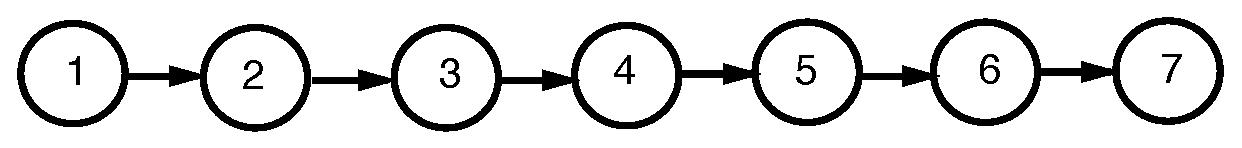
\includegraphics[width=11cm, height=1cm]{images/network_diagram.eps}
				\caption{Сетевой график выполнения работ\label{img:network_diagram}}
			\end{figure}

			Обозначение выполняемых работ:
			\begin{itemize}
				\item 1 --- 2 - формирование требований к ИС (2 дня);
				\item 2 --- 3 - разработка задач ИС и ТЗ (5 дней);
				\item 3 --- 4 - технический проект (14 дней);
				\item 4 --- 5 - рабочая документация, настройка системы и знакомство её с пользователями (4 дня);
				\item 5 --- 6 - ввод в действие (2 дня);
				\item 6 --- 7 - сопровождение АС (15 дней).
			\end{itemize}

			Длительность критического пути составляет $\text{Т}_{\text{кр}}$  = 42 дня.

			\indent Каждый из специалистов задействован на проекте следующее число дней:
			\begin{itemize}
				\item прикладной математик --- 7 дней;
				\item проектировщик --- 13 дней;
				\item разработчик (backend) --- 19 дней;
				\item разработчик (frontend) --- 6 дней;
				\item тестировщик --- 17 дней.
			\end{itemize}

			Затраты по заработной плате рассчитываются следующим образом:
			\begin{equation}\label{eq:salary}
				\text{З} = \text{З}_{\text{зп}} + \text{СВ}
			\end{equation}
				\begin{ESKDexplanation}
				\item[где ]$\text{З}_{\text{зп}}$ --- заработная плата задействованных специалистов, руб.;
				\item $\text{СВ}$ --- страховые взносы во внебюджетные фонды, руб..
			\end{ESKDexplanation}

			\begin{equation}\label{eq:salary_specialist}
				\text{З}_{\text{зп}} = \sum_{i=1}^{n} \frac{ \text{О}_i }{ \text{Д} } * t_i ,		
			\end{equation}
			\begin{ESKDexplanation}
				\item[где ] n --- количество задействованных специалистов, чел.;
				\item $\text{О}_i$ --- оклад i-го специалиста, руб.;
				\item $\text{Д}$ --- количество рабочих дней в месяце, дни;
				\item $t_i$ --- время участия специалиста в проекте (дни), определяется в соответствии с разработанным сетевым планом проектных работ.
			\end{ESKDexplanation}

			Отчисления в Фонд оплаты труда составляют 30\%:
			\begin{equation}\label{eq:royalty}
				\text{СВ} = \text{З}_{\text{зп}} * 0,3
			\end{equation}

			Учитывая разработанные сетевой график и квалификационный план выполнения проектных работ, затраты на заработную плату задействованных специалистов составляют:
			$$\text{З}_{\text{зп}} = 162\,500,00 \text{ руб.}$$

			С полученной суммы в фонд оплаты труда производятся отчисления в размере:
			$$\text{СВ} = 162\,500,00 * 0,3 = 48\,750,00 \text{ руб.}$$

			В итоге затраты по заработной плате состовляют:
			$$\text{З} = 162\,500,00 + 48\,750,00 = 211\,250,00 \text{ руб.}$$

			Основными расходными материалами и нематериальными активами, задействованными при разработке ИС, являются электроэнергия, необходимая для работы компьютеров, и широкополосный доступ в Интернет.

			В процессе разработки  системы задействовано семь компьютеров: по одному на каждого из участиков проекта, один компьютер для разворачивания ИС и один - для запуска СУБД. Средняя номинальная мощность каждого компьютера составляет 100 Вт/ч.

			Затраты на расходные материалы вычисляются по следующей формуле:
			\begin{equation}\label{eq:consumables}
				\text{М} = \text{И} + \text{Э},
			\end{equation}
			\begin{ESKDexplanation}
				\item[где ]$\text{М}$ --- стоимость затраченных расходных материалов, руб.;
				\item $\text{И}$ ---  стоимость услуг интернета, руб.;
				\item $\text{Э}$ ---  стоимость электроэнергии, руб.
			\end{ESKDexplanation}

			Стоимость электроэнергии рассчитывается по следующей формуле:
			\begin{equation}\label{eq:cost_power}
				\text{Э} = \text{Р} * \text{Ц} * \text{Т},
			\end{equation}
			\begin{ESKDexplanation}
				\item[где ]$\text{Р}$ ---  мощность компьютера, кВ;
				\item $\text{Ц}$ ---  цена электроэнергии за кВ.ч, руб..		
			\end{ESKDexplanation}

			Результаты расчета затрат на расходные материалы сведены в таблицу \ref{tab:consumables}.

			\begin{table}[h]
				\small
				\centering
				\caption{Затраты на расходные материалы}
				\label{tab:consumables}								
				\begin{tabular}{|l|l|l|l|}				
				\hline
					\multicolumn{1}{|c|}{Наименование} 										&
					\multicolumn{1}{ c|}{Цена, руб.} 										&
					\multicolumn{1}{ c|}{Количество, ед.} 									&		
					\multicolumn{1}{ c|}{Стоимость, руб (с учетом НДС)} 					\\ \hline
					\multicolumn{1}{|c|}{Электроэнергия} 															&
					\multicolumn{1}{ c|}{3,20}	 																& 
					\multicolumn{1}{ c|}{7 * 0,1 * 12 * 42} 														&
					\multicolumn{1}{ c|}{352,80} 																	\\ \hline
					\multicolumn{1}{|c|}{Интернет} 																&
					\multicolumn{1}{ c|}{4 000,00}																&
					\multicolumn{1}{ c|}{1}																		&
					\multicolumn{1}{ c|}{4 000,00} 																\\ \hline
				\end{tabular}
			\end{table}					

			Амортизация оборудования вычисляется по следующей формуле:
			\begin{equation}\label{eq:amortization}
				A = A_1 + A_2,
			\end{equation}
			\begin{ESKDexplanation}
				\item[где ]$A$ --- общая амортизация, руб.;
				\item $A_1$ --- амортизация ЭВМ, руб.;
				\item $A_2$ --- амортизация сетевого оборудования, руб..
			\end{ESKDexplanation}

			В таблице \ref{tab:norm_amortization} приведены расчеты норм амортизации оборудования, а в таблицу \ref{tab:cost_amortization} сведены затраты на амортизацию оборудования и нематериальных активов, используемых в процессе разработки системы.

			\begin{table}[h]
				\small
				\centering
				\caption{Расчеты норм амортизации оборудования и  программного обеспечения}
				\label{tab:norm_amortization}								
				\begin{tabular}{|l|l|l|l|l|}				
				\hline
					\multicolumn{1}{|c|}{Наименование} 										&
					\multicolumn{1}{ c|}{Стоимость, руб.} 									&
					\multicolumn{1}{ p{3cm}|}{\centering Срок эксплуатации, лет} 			&		
					\multicolumn{1}{ p{3cm}|}{\centering Норма амортизации, руб./мес.} 		&	
					\multicolumn{1}{ p{3cm}|}{\centering Норма амортизации, руб./день} 		\\ \hline
					\multicolumn{1}{|p{3cm}|}{Компьютер} 																&
					\multicolumn{1}{ c|}{70 000,00} 																&
					\multicolumn{1}{ c|}{5}																	&
					\multicolumn{1}{ c|}{1170,00}																	&
					\multicolumn{1}{ c|}{53,00} 																	\\ \hline
					\multicolumn{1}{|p{3cm}|}{Роутеры} 																& 
					\multicolumn{1}{ c|}{5 000,00} 																& 
					\multicolumn{1}{ c|}{5} 																		& 
					\multicolumn{1}{ c|}{83,00} 																	& 
					\multicolumn{1}{ c|}{3,78} 																	\\ \hline
				\end{tabular}
			\end{table}

			\begin{table}[h]
				\small
				\centering
				\caption{Расчет амортизации оборудования и нематериальных активов}
				\label{tab:cost_amortization}								
				\begin{tabular}{|l|l|l|l|l|}				
				\hline
					\multicolumn{1}{|p{3cm}|}{\centeringНаименование} 						&
					\multicolumn{1}{ p{2cm}|}{\centeringКол-во, шт.}						&
					\multicolumn{1}{ p{4cm}|}{\centeringНорма амортизации, руб/день} 		&		
					\multicolumn{1}{ p{3cm}|}{\centeringДлительность, дни} 					&	
					\multicolumn{1}{ p{3cm}|}{\centeringСтоимость, руб.} 					\\ \hline
					\multicolumn{1}{|p{3cm}|}{Компьютер} 																&
					\multicolumn{1}{ c|}{7} 																		& 
					\multicolumn{1}{ c|}{371,00}																	&
					\multicolumn{1}{ c|}{42} 																		& 
					\multicolumn{1}{ c|}{15\,582,00} 																\\ \hline
					\multicolumn{1}{|p{3cm}|}{Роутеры}																& 
					\multicolumn{1}{ c|}{3} 																		& 
					\multicolumn{1}{ c|}{11,34} 																	& 
					\multicolumn{1}{ c|}{42} 																		& 
					\multicolumn{1}{ c|}{476,28} 																	\\ \hline
				\end{tabular}
			\end{table}					

			Исходя из полученных расчётов, стоимость разработки ИС состовялет:
			$$\text{С}_{\text{ис}} = 211\,250,00 + 352,80 + 4\,000,00 +  15\,582,00 + 476,28 = 231\,661,08 \text{ руб.}$$			
		
		\subsubsection{Расчет стоимости выполнения процесса до автоматизации}

			До внедрения ИС процесс проверки работы на плагиат состоит из следующих процессов:
			\begin{itemize}
				\item загрузка работы студента на локальную машину преподавателя;
				\item нахождение работ в системе Moodle для сравнения;
				\item ручная сверка новой работы с другими работами.
			\end{itemize}

			Для расчётов общей стоимости выполнения процесса необходимо расчитать стоимость каждой операции процесса. Стоимость операции рассчитывается как сумма затрат на заработную плату сотрудникам, на амортизацию оброрудования и на расходные материалы:
			\begin{equation}\label{eq:cost_before_automation}
				\text{С}_{\text{до}} = \sum_{i=1}^{n} \text{З}_{Oi} + \sum_{i=1}^{n} \text{М}_{Oi} + \sum_{i=1}^{n} \text{А}_{Oi} ,
			\end{equation}
			\begin{ESKDexplanation}
				\item[где ]$n$ – количество  операций в процессе, штук;
				\item $\text{З}_{Oi}$ --- заработная плата сотрудника при выполнении i-ой операции, руб.;
				\item $\text{М}_{Oi}$ --- затраты на расходные материалы, необходимые при выполнении i-ой операции, руб.;
				\item $\text{А}_{Oi}$ --- амортизация оборудования и нематериальных активов для i-ой  операции, руб..
			\end{ESKDexplanation}	
			
			При выполнении автоматизируемого процесса, как до, так и после автоматизации, затраты на расходные материалы отсутствуют в связи с тем, что все операции производятся исключительно на компьютере пользователя.


			В таблице \ref{tab:salary_before_automation} представлен расчёт затрат на заработную плтату сотрудникам.

			\begin{table}[h]
				\small
				\centering
				\caption{Расчет затрат на заработную плату сотрудникам, выполняющим процесс до автоматизации}
				\label{tab:salary_before_automation}								
				\begin{tabular}{|l|l|l|l|l|}				
				\hline
					\multicolumn{1}{|p{4cm}|}{\centering Операция} 							&
					\multicolumn{1}{ p{3cm}|}{\centering Время выполнения операции, час.} 	&
					\multicolumn{1}{ p{3cm}|}{\centering Зарплтата, руб./час.} 				&		
					\multicolumn{1}{ p{3cm}|}{\centering Количество сотрудников, чел.} 		&	
					\multicolumn{1}{ p{2cm}|}{\centering Затраты, руб.} 					\\ \hline
					\multicolumn{1}{|p{4cm}|}{Загрузка работы студента на локальную машину преподавателя}				& 
					\multicolumn{1}{ c|}{0,10}																	& 
					\multicolumn{1}{ c|}{170,45}																	& 
					\multicolumn{1}{ c|}{1} 																		& 
					\multicolumn{1}{ c|}{22,15}																	\\ \hline
					\multicolumn{1}{|p{4cm}|}{Нахождение работ в системе Moodle для сравнения}		 				& 
					\multicolumn{1}{ c|}{0,20} 																	& 
					\multicolumn{1}{ c|}{170,45} 																	& 
					\multicolumn{1}{ c|}{1}																		& 
					\multicolumn{1}{ c|}{44,31}																	\\ \hline
					\multicolumn{1}{|p{4cm}|}{Ручная сверка новой работы с другими работами}						& 
					\multicolumn{1}{ c|}{3,5}																	& 
					\multicolumn{1}{ c|}{170,45}																	& 
					\multicolumn{1}{ c|}{1}																		&
					\multicolumn{1}{ c|}{775,55} 																	\\ \hline
					Итого & & & & \multicolumn{1}{ c|}{842,01}													\\ \hline
				\end{tabular}
			\end{table}								

			Затарты на амотризацию компьютеров состовляют 123,32 руб.

			$$ \text{С}_{\text{до}} = 965,33 \text{ руб.}$$

		\subsubsection{Расчет стоимости выполнения процесса после автоматизации}

			После внедрения ИС процесс проверки работы на плагиат состоит из следующих процессов:
			\begin{itemize}
				\item просмотр результата проверки работы на плагиат;
				\item ручной запуск проверки на плагиат новой работы;
				\item обработка запроса системой проверки на плагиат;
				\item анализ результата проверки на плагиат.
			\end{itemize}

			Для расчётов общей стоимости выполнения процесса необходимо расчитать стоимость каждой операции процесса. Стоимость операции рассчитывается как сумма затрат на заработную плату сотрудникам и на амортизацию оброрудования:
			\begin{equation}\label{eq:cost_after_automation}
				\text{С}_{\text{после}} = \sum_{i=1}^{n} \text{З}_{Oi} + \sum_{i=1}^{n} \text{М}_{Oi} + \sum_{i=1}^{n} \text{А}_{Oi} ,
			\end{equation}
			\begin{ESKDexplanation}
				\item[где ]$n$ – количество  операций в процессе, штук;
				\item $\text{З}_{Oi}$ --- заработная плата сотрудника при выполнении i-ой операции, руб.;
				\item $\text{М}_{Oi}$ --- затраты на расходные материалы, необходимые при выполнении i-ой операции, руб.;
				\item $\text{А}_{Oi}$ --- амортизация оборудования и нематериальных активов для i-ой  операции, руб..
			\end{ESKDexplanation}

			В таблице \ref{tab:salary_after_automation} представлен расчёт затрат на заработную плтату сотрудникам.

			\begin{table}[h]
				\small
				\centering
				\caption{Расчет затрат на заработную плату сотрудникам, выполняющим процесс после автоматизации}
				\label{tab:salary_after_automation}								
				\begin{tabular}{|C{5cm}|C{2cm}|C{2cm}|C{2cm}|C{3cm}|}				
				\hline
					{Операция} 											&
					{Время выполнения операции, час.} 					&
					{Зарплтата, руб./час.} 								&		
					{Количество сотрудников, чел.} 						&	
					{Затраты, руб.} 									\\ \hline
					\multicolumn{1}{|p{5cm}|}{Просмотр результата проверки работы на плагиат} 							& 
					0,05 																	& 
					170,45 																	& 
					1 																		& 
					8,52 																	\\ \hline
					\multicolumn{1}{|p{5cm}|}{Ручной запуск проверки на плагиат новой работы} 							& 
					0,1 																	& 
					170,45 																	& 
					1 																		& 
					17,05 																	\\ \hline
					\multicolumn{1}{|p{5cm}|}{Анализ результата проверки на плагиат} 									& 
					0,2 																	& 
					170,45 																	& 
					1 																		& 
					34,09 																	\\ \hline 
					\multicolumn{1}{|p{5cm}|}{Итого} & & & & 59,66 													\\ \hline
				\end{tabular}
			\end{table}			

			Затарты на амотризацию компьютеров состовляют 178,73 руб.

		\newpage
		\subsubsection{Расчет экономического эффекта от внедрения подсистемы}
			Годовая экономия рассчитывается по формуле:
			\begin{equation}\label{eq:annual_performance}
				\text{Э} = (\text{С}_{\text{до}} - \text{С}_{\text{после}}) * 100,
			\end{equation}
			$$ \text{Э} = 78\,235,00 \text{руб.}$$

			Годовой экономический эффект рассчитывается по формуле:
			\begin{equation}\label{eq:annual_economic_effect}
				\text{Э}_{\text{г}} = \text{Э} - \text{Е}_{\text{н}} * \text{С}_{\text{ис}},				
			\end{equation}
			\begin{ESKDexplanation}
				\item[где ] Э --- годовая экономия, руб.;
				\item $\text{Е}_{\text{н}}$ --- нормативная эффективность капиталовложений (0,25);
				\item $\text{С}_{\text{ис}}$ --- стоимость разработки подсистемы, руб..
			\end{ESKDexplanation}
			$$\text{Э}_{\text{г}} = 158\,235,00 - 0,25 * 231\,661,08 = 90\,319,73 \text{ руб.}$$

			Исходя из полученных результатов расчета годового экономического эффекта, можно рассчитать коэффициент экономической эффективности:
			\begin{equation}\label{eq:cost_effectiveness_ratio}
				\text{Е} = \text{Э}_{\text{г}} / \text{С}_{\text{ис}},				
			\end{equation}
			\begin{ESKDexplanation}
				\item[где ]$\text{Э}_{\text{г}}$ --- годовой экономический эффект;					
				\item $\text{С}_{\text{ис}}$ --- стоимость разработки подсистемы, руб..
			\end{ESKDexplanation}
			$$\text{Е} = 90\,319,73 / 231\,661,08 = 0,39.$$

			Срок окупаемости данного проекта можно рассчитать по формуле:
			\begin{equation}\label{eq:payback_period}
				\text{Т} = 1 / \text{Е}				
			\end{equation}

			Таким образом, срок окупаемости данного проекта составляет:
			$$\text{Т} = 1 / 0,39 = 2,6 \text{ года}.$$

			Рассчитанные показатели свидетельствуют об экономической эффективности проектируемой ИС <<Шерлок>>.

	\subsection{Инструкция по эксплуатации информационной системы <<Шерлок>>}

		При работе с ИС <<Шерлок>> принимает участие несколько типов пользователей:
		\begin{itemize}
			\item администратор - устанавливает и настраивает работу серверной части ИС (<<backend>>);
			\item сотрудник учебного заведения - взаимодействует с графическим интерфейсом ИС (<<frontend>>);
			\item стороние разработчики - создают сторонние сервисы, которые взаимодействуют с <<backend>>-частью ИС.			
		\end{itemize}

		Далее приведены инструкции для каждого из типов пользователей.

		\subsubsection{Инструкция для администратора}

			ИС <<Шерлок>> распространяется в виде одного jar-файла, который запускается и выполняется на платформе Java, и конфигурационного файла app.config, в котором хранится информация о настройках ИС.

			Перед запуском ИС необходимо установить и настроить следующее ПО на двух рабочих станциях:
			\begin{itemize}
				\item первая рабочая станция - платформа Java (JRE) \cite{web:java}. После установки первая рабочая станция готова к запуску ИС <<Шерлок>>;
				\item вторая рабочая станция - СУБД MongoDB \cite{web:mongodb}. После установки СУБД необходимо произвести её начальную настройку: указать, с каких IP адресов будет доступна база; создать базу данных и пользователя, который имеет доступ к этой БД.
			\end{itemize}

			Перед запуском ИС <<Шерлок>> необходимо настроить систему для работы с БД. Для этого в файле app.properties указывается строка следующего вида:
			$$mongodb://{login}:{password}@{host}/{db},$$
			\begin{ESKDexplanation}
				\item[где ] $\text{login}$ --- логин пользователя для доступа к БД;
				\item $\text{password}$ --- пароль пользователя для доступа к БД;
				\item $\text{host}$ --- адрес машины, на которой работает СУБД;
				\item $\text{db}$ --- название ранее созданой БД.				
			\end{ESKDexplanation}

			Более подробные сведения о подключении к БД можно узнать из документации к Spring Framework \cite{web:mongodb_manual}. После этого система готова к запуску.

			Для запуска ИС на ОС семейства Unix необходимо выполнить следующие действия в консоли:
			\begin{itemize}
				\item перейти в директорию, где располагается файл ИС (sherlock.jar);
				\item запустить ИС следующей командой: $java -jar\ ./sherlock.jar$.
			\end{itemize}

			После этого система запущена и готова к работе.

			Для интеграции Moodle с ИС <<Шерлок>> необходимо произвести установку плагина в соответсвии с инструкцией, распологающейся на оффициальном сайте Moodle.

		\subsubsection{Инструкция для сотрудника учебного заведения}

			Проверка новых студенческих работ на плагиат происходит при загрузке работы студента в Moodle, поэтому при проверке сотрудником работы, ему уже будет доступен результат проверки в виде процентного значения совпадения с другим работами от 0\% до 100\% и ссылка на работу, которая наиболее схожа с проверяемой.

		\subsubsection{Инструкция для разработчиков}

			Несмотря на то, что в рамках данной работы ИС <<Шерлок>> разрабатывается для решения задач в учебной среде, применение ИС не ограничивается только этой средой, а может применятся и в других сферах деятельности человека.

			При проектировании ИС было учтено, что взаимодействие с ней может происходить из совершенно различных систем в плане технической реализации. По этому в качестве реализации интерфейса к ИС (API) был выбран подход REST, который позволяет взаимодействовать с системой посредством обычных HTTP-запросов.

			В таблице \ref{tab:api_method} представлены основные методы взаимодействия с ИС <<Шерлок>>, которые доступны в текущей версии ИС:

			\begin{table}[h]
				\small
				\centering
				\caption{Описание HTTP-методов для взаимодействия с системой}
				\label{tab:api_method}								
				\begin{tabular}{|l|l|p{5cm}|p{5cm}|}				
				\hline
					\multicolumn{1}{|c|}{URL} 												&
					\multicolumn{1}{ c|}{Метод HTTP} 										&
					\multicolumn{1}{ c|}{Описание} 											&		
					\multicolumn{1}{ c|}{Параметры} 										\\ \hline
					/similarity/sync 														& 
					POST 																	& 
					запрос на синхронную проверку работы на плагиат 						&
					sourceText - исходный код проверяемой программы 						\\ \hline
					/similarity/async 														& 
					POST 																	& 
					запрос на асинхронную проверку работы на плагиат. В ответ система генерирует уникальный идетификатор, по которому пользователь в последствии может получить результат проверки &
					sourceText - исходный код проверяемой программы 						\\ \hline
					/similarity/result/ 													& 
					GET 																	& 
					запрос на получение результата проверки на плагиат	 					& 
					uuid - уникальный идентификатор, полученный пользователем при асинхронном запросе на проверку																 \\ \hline
					/user/create 															& 
					POST 																	&
					запрос на создание новой учётной записи пользователя в системе			&
					username - логин нового пользователя; password - пароль нового пользователя \\ \hline
				\end{tabular}
			\end{table}
	\section*{Заключение}
\addcontentsline{toc}{section}{Заключение}

В ближайшем будущем проблема плагиата будет только набирать обороты в связи с всё более широким распространением сети Интернет. Поэтому необходимо уже сейчас разрабатывать меры, которые позволят в дальнейшем не усугубить эту проблему. Одной из таких мер может выступать автоматизация процесса проверки работ на плагиат.

В данной работе было успешно показано, как можно спроектировать и реализовать прототип системы, которая в совокупности с использованием платформы дистанционного обучения позволяет автоматизировать процесс проверки работ на плагиат. После внедрения такой ИС сотруднику учебного заведения достаточно будет пронализировать результаты проверки и принять решение.

Так же стоит заметить, что разработанная ИС является прототипом, который необходимо дорабтать, что бы полностью раскрыть потенциал автоматической проверки работ с помощью информационных технологий. В качестве первостепенных задач для доработки можно выделить разработку интеграционного плагина для ИС <<Moodle>>, добавление поддержки новых языков для проверки и добавление новых алгоритмов для выявления схожести работ. 		
	\bibliographystyle{bibliography/utf8gost705u}
	\bibliography{bibliography/biblio}
	\section*{Приложение А - Исходный код ИС <<Шерлок>>}
\addcontentsline{toc}{section}{Приложение А - Исходный код ИС <<Шерлок>>}

    \lstset{ %
        backgroundcolor=\color{white},   % choose the background color
        basicstyle=\scriptsize,        % size of fonts used for the code
        breaklines=true,                 % automatic line breaking only at whitespace
        captionpos=b,                    % sets the caption-position to bottom
        commentstyle=\color{mygreen},    % comment style
        escapeinside={\%*}{*)},          % if you want to add LaTeX within your code
        keywordstyle=\color{blue},       % keyword style
        stringstyle=\color{mymauve},     % string literal style
        numbers=left,               % где поставить нумерацию строк (слева\справа)
        numbersep=-15pt                % как далеко отстоят номера строк от подсвечиваемого кода
    }

    \begin{lstlisting}[language=java]
        public class SourceCode {
            @Id
            private String id;
            @NotNull
            private String sourceText;
            @NotNull
            private String language;
            private List<String> tokens;
            private String username;
            private String plagiarismProbability;

            public String getId() { return id; }
            public void setId(String id) { this.id = id; }
            public String getSourceText() { return sourceText; }
            public void setSourceText(String sourceText) { this.sourceText = sourceText; }
            public String getLanguage() { return language; }
            public void setLanguage(String language) { this.language = language; }
            public List<String> getTokens() { return tokens; }
            public void setTokens(List<String> tokens) { this.tokens = tokens; }
            public String getUsername() { return username; }
            public void setUsername(String username) { this.username = username; }
            public String getPlagiarismProbability() { return plagiarismProbability; }
            public void setPlagiarismProbability(String plagiarismProbability) { this.plagiarismProbability = plagiarismProbability; }
            @Override
            public String toString() {
                return "SourceCode{" +
                        "sourceText='" + sourceText + '\'' +
                        ", id='" + id + '\'' +
                        ", language='" + language + '\'' +
                        ", tokens=" + tokens +
                        ", username='" + username + '\'' +
                        ", plagiarismProbability=" + plagiarismProbability +
                        '}';
            }
        }
    \end{lstlisting}

    \newpage
    \begin{lstlisting}[language=java]                
        public interface IAlgorithm {
            Float process(List<String> p, List<String> t);
            String getName();
            Float getWeight();
        }
    \end{lstlisting}

    \begin{lstlisting}[language=java]                
        public interface IPreprocessing {
            String process(String sourceText);
        } 
    \end{lstlisting}


    \begin{lstlisting}[language=java]                
        public interface ITokenization {
            Optional<List<String>> process(String sourceText);
        }
    \end{lstlisting}

    \newpage
    \begin{lstlisting}[language=java]                
            public class JavaTokenization implements ITokenization {

            private static Logger log = Logger.getLogger(JavaTokenization.class.getName());

            @Override
            public Optional<List<String>> process(String sourceCode) {
                try {
                    ANTLRInputStream sourceCodeInputStream = new ANTLRInputStream(stringToInputStream(sourceCode));
                    Lexer lexer = new JavaLexer(sourceCodeInputStream);
                    CommonTokenStream commonTokenStream = new CommonTokenStream(lexer);
                    JavaParser parser = new JavaParser(commonTokenStream);
                    IJavaListener listener = new JavaListener();
                    parser.addParseListener(listener);
                    parser.addErrorListener(new BaseErrorListener() {
                        @Override
                        public void syntaxError(Recognizer<?, ?> recognizer, Object offendingSymbol, int line, int charPositionInLine, String msg, RecognitionException e) {
                            throw e;
                        }
                    });
                    parser.compilationUnit();
                    return Optional.of(listener.getTokens());
                } catch (IOException ioe) {
                    log.warning("Error create new ANTLRInputStream(...)");
                    return Optional.empty();
                } catch (RecognitionException re) {
                    log.warning("Recognition error (source code : " + sourceCode.replace("\n", " "));
                    return Optional.empty();
                } catch (Exception e) {
                    log.warning("Unknown error (source code : " + sourceCode.replace("\n", " "));
                    return Optional.empty();
                }
            }

            private InputStream stringToInputStream(String string) {
                return new ByteArrayInputStream(string.getBytes(StandardCharsets.UTF_8));
            }
        }
    \end{lstlisting}


    \newpage
    \begin{lstlisting}[language=java]
        public class RKRGSTAlgorithm implements IAlgorithm {
            private static final Integer MINIMUM_MATCH_LENGTH = 3;        
            private static final Integer INITIAL_SEARCH_LENGTH = 20;
            List<List<MatchValue>> all_matches = new ArrayList<>();
            List<MatchValue> tiles = new ArrayList<>();

            @Override
            public String getName() {
                return "RKR-GST";
            }

            @Override
            public Float getWeight() {
                return 0.5f;
            }

            @Override
            public Float process(List<String> p, List<String> t) {
                    Integer search_length = INITIAL_SEARCH_LENGTH;
                    boolean stop = false;
                    while (!stop) {
                        Integer L_max = scanPattern(search_length, p, t);
                        if (L_max > 2 * search_length)
                            search_length = L_max;
                        else {
                            markStrings(p, t);
                            if (search_length > 2 * MINIMUM_MATCH_LENGTH)
                                search_length = search_length / 2;
                            else if (search_length > MINIMUM_MATCH_LENGTH)
                                search_length = MINIMUM_MATCH_LENGTH;
                            else
                                stop = true;
                        }
                    }
                Float similarity = similarity(p, t, tiles);
                if (similarity > 1.0f){
                    return 1.0f;
                } else {
                    return similarity;
                }
            }

            public Integer scanPattern(Integer search_length, List<String> P, List<String> T) {
                Integer longest_max_match = 0;
                List<MatchValue> matches = new ArrayList<>();
                GSTHashTable hash_table = new GSTHashTable();
                Integer t_position = 0;
                Boolean no_next_tile = false;
                Integer distance;
                while (t_position < T.size()) {
                    if (isMarked(T.get(t_position))) {
                        t_position ++;
                        continue;
                    }
                    Optional<Integer> distance_to_next_tile = distanceToNextTile(t_position, T);
                    if (distance_to_next_tile.isPresent())
                        distance = distance_to_next_tile.get();
                    else {
                        distance = T.size() - t_position;
                        no_next_tile = true;
                    }
                    if (distance < search_length) {
                        if (no_next_tile)
                            t_position = T.size();
                        else {
                            if (jumpToNextUnmarkedTokenAfterTile(t_position, T).isPresent())
                                t_position = jumpToNextUnmarkedTokenAfterTile(t_position, T).get();
                            else
                                t_position = T.size();
                        }
                    } else {
                        String t_substring = T.subList(t_position, t_position + search_length).stream().collect(Collectors.joining());
                        hash_table.put(hash(t_substring), t_position);
                        t_position ++;
                    }
                }
                no_next_tile = false;
                Integer p_position = 0;
                while (p_position < P.size()) {
                    if (isMarked(P.get(p_position))) {
                        p_position ++;
                        continue;
                    }
                    Optional<Integer> distance_to_next_tile = distanceToNextTile(p_position, P);
                    if (distance_to_next_tile.isPresent())
                        distance = distance_to_next_tile.get();
                    else {
                        distance = P.size() - p_position;
                        no_next_tile = true;
                    }
                    if (distance < search_length) {
                        if (no_next_tile)
                            p_position = P.size();
                        else {
                            if(jumpToNextUnmarkedTokenAfterTile(p_position, P).isPresent())
                                p_position = jumpToNextUnmarkedTokenAfterTile(p_position, P).get();
                            else {
                                p_position = P.size();
                            }
                        }
                    } else {
                        String p_substring = P.subList(p_position, p_position + search_length).stream().collect(Collectors.joining());
                        ArrayList<Integer> positions = hash_table.get(hash(p_substring));
                        for (Integer position : positions) {
                            String t_substring = T.subList(position, position + search_length).stream().collect(Collectors.joining());
                            if (t_substring.equals(p_substring)) {
                                t_position = position;
                                Integer k = search_length;
                                while (p_position + k < P.size() && t_position + k < T.size()
                                        && P.get(p_position + k).equals(T.get(t_position + k))
                                        && isUnmarked(P.get(p_position + k))
                                        && isUnmarked(T.get(t_position + k)))
                                    k ++;
                                if (k > 2 * search_length)
                                    return k;
                                else {
                                    if (longest_max_match < search_length)
                                        longest_max_match = search_length;
                                    matches.add(new MatchValue(p_position, t_position, k));
                                }
                            }
                        }
                        p_position ++;
                    }
                }
                if (!matches.isEmpty()){
                    all_matches.add(matches);
                }
                return longest_max_match;
            }

            private void markStrings(List<String> p, List<String> t) {
                all_matches.forEach(matches -> matches.stream().filter(match -> !isOccluded(match, tiles)).forEach(match -> {
                    IntStream.range(0, match.getLengthMatch()).forEach(i -> {
                        Integer pattern_position = match.getPatternPosition() + i;
                        Integer text_position = match.getTextPosition() + i;
                        p.set(pattern_position, markToken(p.get(pattern_position)));
                        t.set(text_position, markToken(t.get(text_position)));
                    });
                    tiles.add(match);
                }));
                all_matches.clear();
            }

            private static Long hash(String string) {
                AtomicLong hash = new AtomicLong(0);
                string.chars().forEach(symbol -> hash.set((hash.intValue() << 1) + symbol));
                return hash.longValue();
            }

            private Boolean isUnmarked(String string) {
                return string.length() > 0 && string.charAt(0) != '*';
            }

            private Boolean isMarked(String string) {
                return (!isUnmarked(string));
            }

            private String markToken(String string) {
                return "*" + string;
            }

            private Boolean isOccluded(MatchValue match_value, List<MatchValue> tiles) {
                return tiles.stream().anyMatch(tile -> (tile.getPatternPosition() + tile.getLengthMatch() == match_value.getPatternPosition() + match_value.getLengthMatch()) && (tile.getTextPosition() + tile.getLengthMatch() == match_value.getTextPosition() + match_value.getLengthMatch()));
            }

            private Optional<Integer> distanceToNextTile(Integer current_position, List<String> tokens) {
                Integer distance_to_next_tile = (int) StreamUtils.takeWhile(tokens.stream().skip(current_position + 1), this::isUnmarked).count();
                return current_position + distance_to_next_tile + 1 != tokens.size() ? Optional.of(distance_to_next_tile + 1) : Optional.empty();
            }

            private Optional<Integer> jumpToNextUnmarkedTokenAfterTile(Integer current_position, List<String> tokens) {
                Optional<Integer> position_after_next_tile = Optional.empty();
                Optional<Integer> distance_to_next_tile = distanceToNextTile(current_position, tokens);
                if (distance_to_next_tile.isPresent()) {
                    Integer count_marked_tokens = (int) StreamUtils.takeWhile(tokens.stream().skip(current_position + distance_to_next_tile.get() + 1), this::isMarked).count();
                    if (current_position + distance_to_next_tile.get() + count_marked_tokens + 1 <= tokens.size() - 1) {
                        position_after_next_tile = Optional.of(current_position + distance_to_next_tile.get() + count_marked_tokens + 1);
                    }
                }
                return position_after_next_tile;
            }

            private Float similarity(List<String> p, List<String> t, List<MatchValue> tiles) {
                return (float) (2 * coverage(tiles)) / (float) (p.size() + t.size());
            }

            private Integer coverage(List<MatchValue> tiles) {
                return tiles.stream().collect(Collectors.summingInt(MatchValue::getLengthMatch));
            }
        }
        
    \end{lstlisting}  

    \newpage
    \begin{lstlisting}[language=java]
        @Configuration
        @ComponentScan
        @RestController
        @RequestMapping(value = "/sherlock/api")
        public class SimilarityController {
            private static Logger log = Logger.getLogger(SimilarityController.class.getName());
            @Autowired
            private SimilarityService similarityService;
            @Autowired
            private SourceCodeRepository sourceCodeRepository;

            @RequestMapping(method = RequestMethod.POST, value = "/similarity/sync")
            public ResponseEntity<ApiResponse> syncSimilarity(@Valid @RequestBody SourceCode sourceCode, Principal user) {
                log.info(String.join(" : ", "/sherlock/api/similarity/sync", user.getName(), sourceCode.toString()));
                sourceCode.setUsername(user.getName());
                Optional<Float> plagiarismProbability = similarityService.syncProcess(sourceCode);
                if (plagiarismProbability.isPresent()) {
                    return new ResponseEntity<>(new ApiResponse(plagiarismProbability.get().toString()), HttpStatus.OK);
                } else {
                    return new ResponseEntity<>(HttpStatus.BAD_REQUEST);
                }
            }

            @RequestMapping(method = RequestMethod.POST, value = "/similarity/async")
            public ResponseEntity<ApiResponse> asyncSimilarity(@Valid @RequestBody SourceCode sourceCode, Principal user) {
                log.info(String.join(" : ", "/sherlock/api/similarity/async", user.getName(), sourceCode.toString()));
                sourceCode.setUsername(user.getName());
                String uuid = UUID.randomUUID().toString();
                similarityService.asyncProcess(sourceCode, uuid);
                return new ResponseEntity<>(new ApiResponse(uuid), HttpStatus.OK);
            }

            @RequestMapping(method = RequestMethod.GET, value = "/similarity/result/{uuid}")
            public ResponseEntity<ApiResponse> resultSimilarity(@PathVariable String uuid) {
                SourceCode search_source_code = sourceCodeRepository.findOne(uuid);
                if (search_source_code != null) {
                    return new ResponseEntity<>(new ApiResponse(search_source_code.getPlagiarismProbability()), HttpStatus.OK);
                } else {
                    return new ResponseEntity<>(HttpStatus.BAD_REQUEST);
                }
            }

            @InitBinder("sourceCode")
            protected void initBinder(WebDataBinder binder) {
                binder.setValidator(new SourceCodeValidator());
            }
        }

    \end{lstlisting}

    \newpage
    \begin{lstlisting}[language=java]
        @RestController
        @RequestMapping(value = "/sherlock/api")
        public class UserController {

            private AccountService accountService;

            @Autowired
            public UserController(AccountService accountService) {
                this.accountService = accountService;
            }

            @RequestMapping(method = RequestMethod.POST, value = "/user/create")
            public ApiResponse createUser(@Valid @RequestBody Account account) {
                if (accountService.create(account).isPresent()) {
                    return new ApiResponse("OK");
                } else {
                    return new ApiResponse("ERROR");
                }
            }

            @InitBinder
            protected void initBinder(WebDataBinder binder) {
                binder.setValidator(new AccountValidator());
            }
        }
    \end{lstlisting}

    \newpage
    \begin{lstlisting}[language=java]
        @Service
        public class AccountServiceImpl implements AccountService {

            private AccountRepository accountRepository;

            @Autowired
            public AccountServiceImpl(AccountRepository accountRepository) {
                this.accountRepository = accountRepository;
            }

            @Override
            public Optional<Account> getAccountByUsername(String username) {
                return Optional.ofNullable(accountRepository.findByUsername(username));
            }

            @Override
            public Optional<Account> create(Account account) {
                if (accountRepository.findByUsername(account.getUsername()) == null) {
                    account.setPasswordHash(new BCryptPasswordEncoder().encode(account.getPassword()));
                    account.setRole(Role.ROLE_USER);
                    return Optional.of(accountRepository.save(account));
                } else {
                    return Optional.empty();
                }
            }
        }    
    \end{lstlisting}

    \newpage
    \begin{lstlisting}[language=java]
        public interface AccountRepository extends MongoRepository<Account, String> {
            Account findByUsername(String username);
        }
    \end{lstlisting}

    \begin{lstlisting}[language=java]
        public class ApiResponse {
            private String message;

            public ApiResponse() { }

            public ApiResponse(String message) {
                this.message = message;
            }
            public String getMessage() {
                return message;
            }
        }
    \end{lstlisting}

    \newpage
    \begin{lstlisting}[language=java]
        public class Account {
            @Id
            private String id;
            private String username;
            @Transient
            private String password;
            private String passwordHash;
            private Role role;

            public Account() { }
            public Account(String username, String passwordHash, Role role) {
                this.username = username;
                this.passwordHash = passwordHash;
                this.role = role;
            }

            public String getId() {
                return id;
            }
            public void setId(String id) {
                this.id = id;
            }
            public String getUsername() {
                return username;
            }
            public void setUsername(String username) {
                this.username = username;
            }
            public String getPassword() {
                return password;
            }
            public void setPassword(String password) {
                this.password = password;
            }
            public String getPasswordHash() {
                return passwordHash;
            }
            public void setPasswordHash(String passwordHash) {
                this.passwordHash = passwordHash;
            }
            public Role getRole() {
                return role;
            }
            public void setRole(Role role) {
                this.role = role;
            }
        }
    \end{lstlisting}

    \newpage
    \begin{lstlisting}[language=java]
        @EnableWebSecurity
        @Configuration
        @Order(SecurityProperties.ACCESS_OVERRIDE_ORDER)
        public class SecurityConfig extends WebSecurityConfigurerAdapter {
            @Autowired
            UserDetailsService userDetailsService;
            @Override
            protected void configure(HttpSecurity http) throws Exception {
                http
                    .csrf().disable()
                    .sessionManagement().sessionCreationPolicy(SessionCreationPolicy.STATELESS)
                    .and()
                    .authorizeRequests()
                    .antMatchers("/sherlock/api/user/**").hasAuthority(Role.ROLE_ADMIN.name())
                    .antMatchers("/sherlock/api/check/**").hasAuthority(Role.ROLE_USER.name())
                    .and()
                    .httpBasic();
            }

            @Override
            public void configure(AuthenticationManagerBuilder auth) throws Exception {
                auth
                        .userDetailsService(userDetailsService)
                        .passwordEncoder(new BCryptPasswordEncoder());
            }

            @Bean
            UserDetailsService getUserDetailsService() {
                return new UserDetailsService() {
                    @Autowired
                    private AccountService accountService;

                    @Override
                    public UserDetails loadUserByUsername(String username) throws UsernameNotFoundException {
                        Account account = accountService.getAccountByUsername(username)
                                .orElseThrow(() -> new UsernameNotFoundException(String.format("User with username=%s was not found", username)));

                        return new User(account.getUsername(),
                                        account.getPasswordHash(),
                                        true,
                                        true,
                                        true,
                                        true,
                                        AuthorityUtils.createAuthorityList(account.getRole().name()));
                    }
                };
            }
        }
    \end{lstlisting}    

    \newpage
    \begin{lstlisting}[language=java]
        @SpringBootApplication
        public class Application {
            public static void main(String[] args) {
                SpringApplication.run(Application.class, args);
            }
        }
    \end{lstlisting}
	\section*{Приложение Б - Псевдокод алгоритма RKR-GST}
\addcontentsline{toc}{section}{Приложение Б - Псевдокод алгоритма RKR-GST}

Псевдокод для основного тела алгоритма
\newline
\begin{algorithm}[H]
	\SetAlgoLined %% Это соединяет линиями логические части

	search-length s := initial-search-length;

	stop := false;

	\Repeat{stop} {
		$L_{max}$ := scanpattern(s);

		\eIf{$L_{max}$ > 2 $\times$ s}{
			s := $L_{max}$;
		}{
			markstrings(s);

			\eIf{s > 2 $\times$ minimum\_match\_length}{
				s := s div 2;
			}{
				\eIf{s > minimum\_match\_length}{
					s := $minimum\_match\_length$;
				}{
					stop := true;
				}	
			}
		}
	}		
\end{algorithm}

\newpage
Псевдокод для функции $scanpattern()$
\newline
\begin{algorithm}[H]
	\small
	\SetAlgoLined

	\For{unmarked tokens $T_t$}{
		\eIf{distance to next tile $\le$ s}{
			advance $t$ to first unmarked token after next tile;
		}{
			create the KR hash-value for substring $T_t$ . . . $T_{t + s - 1}$ and add to hashtable;	
		}	
	}


	\For{unmarked tokens $P_p$}{
		\eIf{distance to next tile $\le$ s}{
			advance $p$ to first unmarked token after next tile;
		}{
			create the KR hash-value for substring $P_p$ . . . $P_{p + s - 1}$ and add to hashtable;

			check hashtable for hash of KR hash-value;

			\For{each hash-table entry with equal hashed KR hash-value}{
				
				k := s;

				\While{$P_{p + k} = T_{t + k} \ \& \ unmarked(P_p + k) \ \& \ unmarked(T_t + k)$}{
					k := k + 1;
				}
				\eIf{k > 2 $\times$ s}{
					return(k);
				}{
					record new maximal-match;			
				}	
			}
		}	
	}
	return(length of longest maximal-match);
\end{algorithm}

\newpage
Псевдокод для функции $markstrings()$
\newline
\begin{algorithm}[H]
	\small
	\SetAlgoLined

	\While{$queue\ non-empty$}{
		\eIf{$current\ queue\ is\ empty$}{
			drop to next queue;
		}{
			remove match(p, t, L) from queue;

			\eIf{$match\ not\ occluded$}{
				\For{$j\leftarrow 0$ \KwTo $s-1$}{
					\eIf{$P_{p+j} = T_{t+j}$}{
						\For{$i\leftarrow 0$ \KwTo $s-1$}{
							mark\_token($P_{p + i}$);

							mark\_token($T_{p + i}$);
						}

						$length\_of\_tokens\_tiled := length\_of\_tokens\_tiled + L$;
					}							
				}		
			}{
				\eIf{$L - L_{occluded} \ge s $}{
					replace unmarked portion on list of queues;
				}			
			}	
		}	
	}
 \end{algorithm}

			
\end{document}